\documentclass[pdftex,11pt,a4paper]{book}

\usepackage[utf8]{inputenc}
\usepackage[spanish]{babel}
\usepackage[latin1]{inputenc}
\usepackage[pdftex]{graphicx}
\usepackage{url}
\usepackage[top=1.5in, bottom=1in, left=1in, right=1in]{geometry}
\usepackage{hyperref}
\usepackage{multirow}

\usepackage{eurosym}  
\DeclareUnicodeCharacter{20AC}{\euro}

\usepackage{float}
\usepackage{array}
\usepackage{tabularx}
\usepackage{longtable}

\usepackage[usenames]{color}

\newcommand{\HRule}{\rule{\linewidth}{0.5mm}}

\usepackage{verbatimbox}
\newcommand\Includegraphics[2][]{\addvbuffer[12pt 6pt]{\includegraphics[#1]{#2}}}

\begin{document}

\begin{titlepage}
\begin{center}

% Upper part of the page. The '~' is needed because \\
% only works if a paragraph has started.
% -----

\includegraphics[width=0.15\textwidth]{logoUJI.jpg}~\\[2cm]

\textsc{\LARGE Grado en Ingeniería Informática}\\[1.5cm]

\textsc{\LARGE Trabajo de Final de Grado}\\[1.5cm]
%%%%%%\textsc{\LARGE Versión Provisional}\\[1.5cm]

% Title
\HRule \\[0.4cm]
{ \huge \bfseries Aplicación web para la consulta del consumo de agua \\[0.4cm] }

\HRule \\[1.5cm]

% Author and supervisor
\begin{minipage}{0.4\textwidth}
\begin{flushleft} \large
\emph{Autor:}\\
Rosa María \textsc{de Juan Oliva}
\end{flushleft}
\end{minipage}
\begin{minipage}{0.4\textwidth}
\begin{flushright} \large
\emph{Supervisor:} \\
Jose Luís \textsc{Martínez Pérez} \\
\emph{Tutor académico:} \\
María de las Mercedes \textsc{Fernández Redondo}
\end{flushright}
\end{minipage}

\vfill

% Bottom of the page
% -----
% Sustituir los signos "\_" por lo que corresponda. 
{\large Fecha de lectura: \_\_ de \_\_\_\_\_\_\_\_\_ de 20\_\_\\
Curso académico 20\_\_/20\_\_}

\end{center}
\end{titlepage}
\setlength{\parskip}{\baselineskip}



% ------------------- Página resumen ---------------------

\thispagestyle{empty} % página sin numerar

\clearpage % Resumen y Palabras clave en página 2.

\section*{Resumen}

Este documento contiene la memoria del trabajo de final de grado en el que se expone el desarrollo de una aplicación web para la consulta del consumo de agua de los clientes abonados y la gestión de alarmas en sus contadores con el fin de detectar problemas o fugas. Esta aplicación va dirigida tanto a clientes particulares como a empresas, aunque esta memoria se centra en el desarrollo de la parte del cliente particular.

El \textit{frontend} de la aplicación se ha implementado utilizando el \textit{framework} Angular 8 y el lenguaje de programación \textit{Typescript}. Por el contrario, para el \textit{backend} se ha empleado el \textit{framework Spring} y el lenguaje de programación \textit{Java}.


\section*{Palabras clave}

Contadores, consumo de agua, aplicación web, Angular, Spring framework.

\section*{Keywords}

\textit{Water meters, water consumption, web application, Angular, Spring framework.}

\thispagestyle{empty} % página sin numerar

\cleardoublepage



% ------------------- Página índice ---------------------

\pagestyle{plain} % todas las páginas numeradas, sin cabeceras. Sustituir por \pagestyle{headings} para añadir cabeceras a las páginas. 

\tableofcontents
\addcontentsline{bib}{bibliography}{Bibliografía}


\cleardoublepage
\listoffigures
\listoftables

\cleardoublepage



% ------------------- Página explicativa, no debe constar en la memoria ---------------------

% ---- BORRAR DESDE AQUÍ

% El apartado borrado aquí es el de las instrucciones, lo tengo guardado aparte.

% ---- BORRAR HASTA AQUÍ



% ------------------- Cuerpo de la memoria ---------------------

\chapter{Introducción} \label{capitulo:introduccion}

\section{Contexto y motivación del proyecto}

El proyecto documentado en esta memoria se desarrolló en la empresa IoTsens. Esta empresa se dedica a la venta de soluciones software e IoT a medida para la gestión de datos, ofreciendo también soporte y mantenimiento de las mismas \cite{bib:IoTsens}. La empresa IoTsens forma parte de Grupo Gimeno, un conjunto de empresas de varios sectores que tienen como objetivo la innovación, el desarrollo sostenible y la mejora de la calidad de vida de los ciudadanos e industrias \cite{bib:grupo-gimeno}.

A raíz de una idea surgida durante el Hackathon 2019 de la Universitat Jaume I, la cual consistía en una aplicación que gestionara la recogida de residuos de una ciudad de forma inteligente, se decidió proponer su desarrollo a la empresa IoTsens. Esto fue posible gracias a las profesoras María Asunción Castaño Álvarez y Lledó Museros Cabedo, quienes facilitaron el contacto con Ignacio Llopis, director gerente de IoTSens. 
Finalmente, se decidió el desarrollo de una aplicación con objetivos similares, pero enfocada a la consulta del consumo de agua. El progreso de este proyecto, desde el inicio de su propuesta hasta parte de su implementación, es el que se desarrolla en esta memoria.

La realización de este proyecto viene dada por la necesidad de proporcionar a clientes particulares una plataforma donde poder visualizar información sobre su consumo de agua en un formato fácil de comprender, con el fin de hacer un uso responsable de la misma. También se quería poder detectar y controlar las posibles fugas o problemas que tuviera un contador lo más rápido posible para poder tomar medidas en consecuencia.

Otros de los motivos por los que se decidió desarrollar este proyecto fue el hecho de disponer de una aplicación parecida llamada \textit{Smart Water}\footnote{La información de esta aplicación se encuentra en el enlace: \url{www.iotsens.com/solucion/smart-water/}}, la cual ya estaba implementada y enfocada a los profesionales del sector de la gestión del ciclo del agua, pero no a los clientes particulares o a grandes consumidores.


\section{Objetivos del proyecto} \label{seccion:objetivos}

El objetivo principal de este proyecto consiste en la creación de una aplicación que permita al usuario llevar un control sobre sus contadores y su consumo de agua de manera sencilla. Este objetivo, se puede desglosar en los siguientes:

\begin{itemize}
\item Permitir que el usuario pueda consultar su consumo de agua
\item Visualizar de manera gráfica y fácilmente comprensible la lectura y consumo de un contador.
\item Permitir que el usuario gestione las alarmas de sus contadores y que éstas le informen en caso de algún problema.
\item Posibilitar las predicciones de consumo de agua
\end{itemize}

Los principales beneficios que conllevaría la existencia de una aplicación de este tipo serían el consumo más responsable de agua, así como una mejor gestión y conocimiento sobre ello por parte de clientes particulares.


\section{Descripción del proyecto}

A continuación, se explica con más detalle los requisitos especificados para la aplicación web desarrollada durante la estancia en prácticas, llamada \textit{Water Clients}.

En primer lugar, el sistema debe permitir la autentificación de los clientes para poder acceder a la aplicación, así como desconectarse de la misma.

En segundo lugar, el sistema debe mostrar los datos de los contadores que tenga el cliente, así como su consumo. Por una parte, esto incluye la visualización de la póliza, código y dirección de un contador. A su vez, el sistema debe mostrar las gráficas de consumo de agua y lecturas en un período de tiempo e intervalos especificados por el cliente. También debe permitir la visualización del consumo diario promedio del contador, el consumo hecho a lo largo del día y la diferencia con respecto al día anterior.

El sistema también debe permitir que el cliente pueda añadir, modificar o desactivar alarmas para uno o varios contadores. Esto incluye la posibilidad de que el cliente pueda especificar el tipo de alarma y un período de tiempo determinado en el que esté activa.

Además, el cliente debe tener la posibilidad de añadir datos adicionales sobre el contexto en el que se encuentra su contador, como es la cantidad de baños que tiene la vivienda, cantidad de personas, si se dispone de lavavajillas o lavadora, etc.

Por otro lado, el sistema debe permitir al administrador gestionar las cuentas de sus clientes, así como ver la información de sus contadores y alarmas.

Finalmente, el cliente debe poder visualizar en un mapa interactivo la ubicación de sus contadores.

Adicionalmente, a modo de mejora, se debe tener en cuenta que el sistema pueda mostrar estadísticas sobre el consumo de agua de un contador a partir de los datos adicionales proporcionados por el cliente. Aunque esto queda fuera del alcance funcional del proyecto.

Cabe mencionar que la parte del sistema relacionada con la administración de usuarios no se incluye en esta memoria, puesto que fue implementada por otro miembro del equipo de desarrollo. Tampoco se incluye la gestión de alarmas, a excepción de las consultas, por la misma razón mencionada anteriormente. En la sección \ref{seccion:planificacion} se explica en detalle el porqué de este hecho.


\section{Estructura de la memoria}

El contenido de esta memoria está organizado en varios capítulos, comentados a continuación.

El capítulo 1 explica la motivación, los objetivos y de qué trata el proyecto que se ha realizado durante la estancia en prácticas. También se describe brevemente la empresa donde se ha llevado a cabo.

En el capítulo 2 se muestra la planificación que se ha seguido para llevar a cabo el desarrollo del proyecto, así como la estimación de recursos, las tecnologías utilizadas y la metodología adoptada.

El capítulo 3 se lleva a cabo la definición de los requisitos del sistema y explica la arquitectura del mismo. A su vez analiza el diseño de la interfaz gráfica de la aplicación. 

El capítulo 4 se centra en la implementación de la aplicación llevada a cabo y los resultados obtenidos.

En el capítulo 5 se muestran las pruebas de aceptación diseñadas para validar el sistema y se comentan las pruebas unitarias y de integración realizadas. 

El capítulo 6 trata de las reflexiones sobre el proyecto llevado a cabo y la estancia en prácticas.


%################# CAPÍTULO 2 - PLANIFICACIÓN DEL PROYECTO ##############################

\chapter{Planificación del proyecto} \label{capitulo:planificacion}

% -------------------
\section{Metodología} \label{seccion:metodologia}

Debido a la naturaleza de este proyecto, sujeto a la posibilidad de cambios y mejoras en algunos de sus aspectos menos definidos, se optó por seguir la metodología ágil \textit{Kanban}, con algunos matices propios de la metodología \textit{Scrum}. Para poder analizar mejor en qué consistió esta agrupación de ambas metodologías, es necesario definirlas antes.

Por un lado, la metodología ágil \textit{Kanban} tiene como objetivo la gestión eficiente del tiempo y el trabajo, ayudando a limitar la acumulación de las tareas pendientes y generando un flujo de trabajo constante y equilibrado \cite{bib:kanban}. Para ayudar a visualizar ello, se dispone del tablero \textit{Kanban}, el cual se divide en diversos estados. Las tareas van pasando por cada uno de ellos hasta quedar finalizadas. La cantidad de estados puede variar dependiendo del tipo de proyecto y su complejidad.

Por otra parte, la metodología Scrum se caracteriza por dividir la realización de un proyecto en pequeños ciclos temporales de duración fija llamados iteraciones. Al final de cada una de ellas se realiza una reunión para dar un feedback del resultado. Las tareas a completar se suelen medir según su prioridad y complejidad \cite{bib:scrum}.

Para la realización de este proyecto, se estableció una pila del producto para poder determinar la complejidad de cada funcionalidad a implementar y su prioridad. Además, se planificaron reuniones semanales para el seguimiento del proyecto. A su vez, se dispuso de un tablero \textit{Kanban} donde se podía visualizar el estado de cada tarea en todo momento.


% ----------------------
\section{Tecnología} \label{seccion:tecnologia}

A la hora de hablar de las tecnologías que se utilizaron en la elaboración del código, de debe distinguir entre dos partes bien diferenciadas: \textit{frontend} y \textit{backend}. La primera hace referencia a la parte web de la aplicación, la capa de presentación, aquella que interactúa con los usuarios \cite{bib:front-end}. Por contra, la capa de acceso a datos, el \textit{backend}, es la encargada de interactuar con el servidor, la base de datos u otras aplicaciones con el objetivo de procesar la información proveniente tanto de alguno de los tres anteriores para enviarla al \textit{frontend} y viceversa \cite{bib:frontendybackend}.

En primer lugar, con respecto a la implementación del \textit{frontend}, se utilizó el \textit{framework}\footnote{Es un marco de trabajo cuya estructura o esquema establecido se utiliza para desarrollar \textit{software} \cite{bib:framework}.} \textit{Angular}, concretamente la versión 8, una de las más recientes. Este \textit{framework} incluye el uso del lenguaje de programación \textit{Typescript} y los lenguajes de etiquetas \textit{HTML} y \textit{CSS}, con los cuales se obtuvo una interfaz gráfica cómoda y agradable, a la vez que un código bien estructurado. Además, en relación a la interfaz de usuario, para lograr que ésta fuera \textit{responsive}\footnote{Capacidad para redimensionar el contenido de la aplicación de manera coherente para adaptarse a diferentes dispositivos electrónicos, cuyos tamaños son variados \cite{bib:responsive}.}, se utilizó otro \textit{framework} llamado \textit{Bootstrap}.

Con respecto al \textit{backend}, se usó \textit{Spring}, el cual es un \textit{framework} de código abierto para el desarrollo de aplicaciones con \textit{Java} \cite{bib:spring}, cuyo lenguaje de programación se utilizó conjuntamente con este \textit{framework}. El uso de \textit{Spring} simplificó las configuraciones iniciales, el acceso a la base de datos y las consultas a los microservicios de IoTsens.  

También, cabe destacar la parte de las posibles mejoras que se plantearon para la aplicación. Estas mejoras están relacionadas con el análisis predictivo a modo de introducción al \textit{machine learning}, que es la disciplina perteneciente al ámbito de la IA (Inteligencia Artificial) focalizada en el aprendizaje automático \cite{bib:machine-learning}. Para poder llevar a cabo su implementación en un futuro, se decidió estudiar el uso de \textit{Python}, así como de \textit{R}. Esto se debió a que ambos lenguajes de programación tienen librerías muy populares para \textit{machine learning}, con un gran soporte técnico y documentación.

En relación con los recursos de \textit{hardware} utilizados durante el desarrollo del proyecto, sólo se requirió de un ordenador de sobremesa para cada miembro del equipo. Aunque durante el estado de alarma debido al COVID-19, se tuvieron que usar los ordenadores personales.

% ----------------------------
\section{Herramientas}

Para este proyecto se utilizaron una serie de herramientas con la finalidad de ayudar en la correcta gestión, documentación desarrollo del mismo, así como para mantener una buena comunicación dentro del equipo de trabajo.

% ............
\subsection{Herramientas de gestión y documentación} 

Inicialmente, se usó la herramienta \textit{Jira Software}, una plataforma web que ayuda en la planificación, desarrollo, gestión y supervisión de proyectos software ágiles \cite{bib:atlassian}. Dispone de un tablero \textit{Kanban} para visualizar el flujo de trabajo y hacer un seguimiento de las tareas, lo que hizo tener una visión general del avance del proyecto en todo momento. La figura \ref{fig:tablero-kanban} muestra el tablero \textit{Kanban} utilizado durante la implementación del proyecto.

\begin{figure}[H]
 \centering
 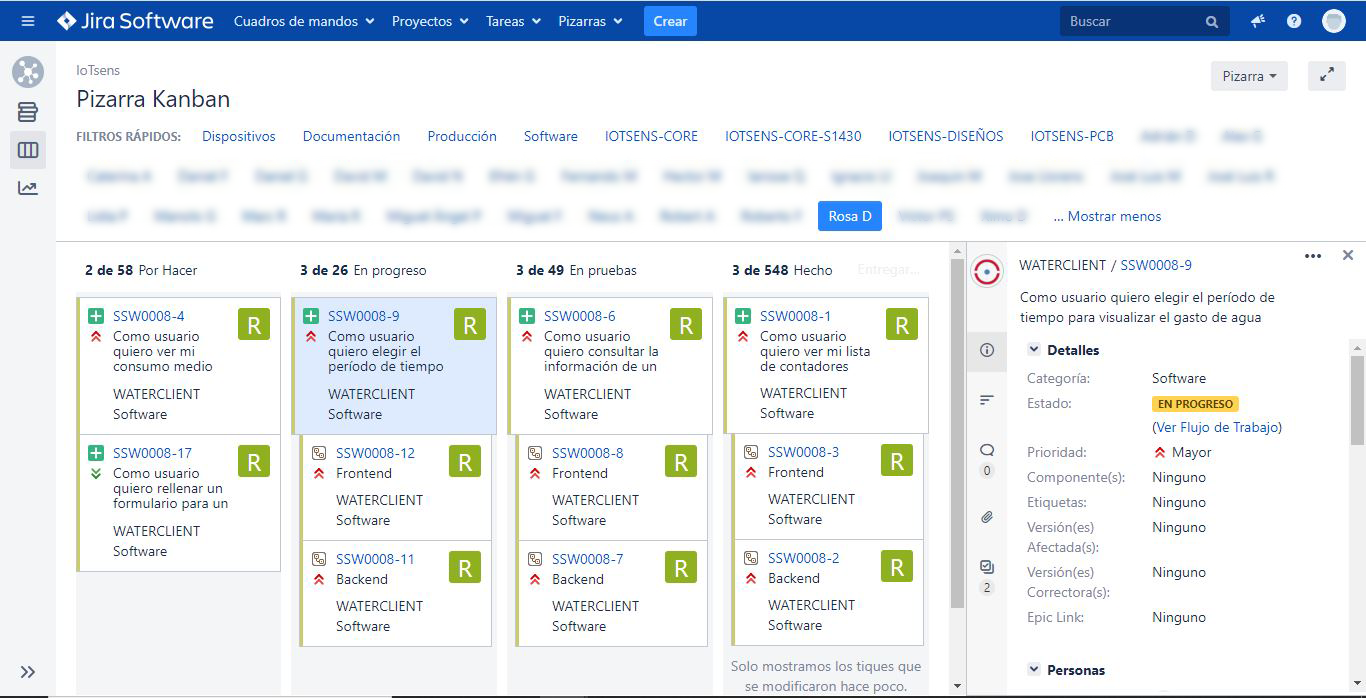
\includegraphics [scale=0.42] {images/planificacion/kanban.png}
 \caption{Tablero \textit{Kanban}} \label{fig:tablero-kanban}
 \end{figure}

Puesto que la herramienta \textit{Jira Software} está especializada en el desarrollo de proyectos informáticos, ésta permite la creación de tareas de diferente tipo relacionadas con la implementación de funcionalidades de una aplicación. El tipo de tarea más común es la historia de usuario,la cual hace referencia a los requisitos y funcionalidades de un sistema informático expresadas desde el punto de vista del usuario final que quiere utilizar dicho sistema. También están las épicas, que son historias de usuario de gran tamaño que se descomponen en varias de tamaño menor para poder ser gestionadas individualmente \cite{bib:epica-HU}. Por otro lado, se pueden crear tareas que indiquen errores.

Asimismo, es posible detallar las diferentes tareas creadas añadiéndoles descripción, prioridad, puntos de historia\footnote{Medida subjetiva para estimar la complejidad de una tarea \cite{bib:puntos-historia}.} y subtareas. Cada una puede ser asignada al miembro del equipo responsable de realizarla y/o al responsable de su supervisión.


Por otra parte, cabe destacar que \textit{Jira} permite también la creación y gestión de esprints, que son propios de la metodología ágil \textit{Scrum}. A pesar de que en este proyecto no se realizaron esprints, es importante tener en cuenta esta posibilidad, ya que es otra forma más de facilitar la combinación de las metodologías ágiles \textit{Scrum} y \textit{Kanban}, de las cuales se utilizaron elementos de ambas para el desarrollo de este proyecto, como se explica en la sección \ref{seccion:metodologia}.

Otra herramienta utilizada fue \textit{Confluence}, con el fin de consultar la documentación de los diferentes microservicios creados por la empresa y utilizados para la obtención de diferentes tipos de mediciones de dispositivos y alarmas. \textit{Confluence} es una wiki\footnote{Plataforma web que se utiliza para la colaboración, documentación y recopilación de información \cite{bib:wiki}.} utilizada en entornos corporativos para la colaboración en equipo \cite{bib:wiki}. Esta herramienta fue imprescindible, puesto que se usaron varias de estos microservicios ya documentados en esta plataforma para la implementación de la aplicación \textit{Water Clients}. Cabe añadir que \textit{Confluence} también permite redactar informes sobre la evolución y reuniones que se han realizado a lo largo del desarrollo de un proyecto, para poder tener un seguimiento bastante preciso del mismo.

Finalmente, cabe destacar que, debido a situación derivada a causa del COVID-19, se pasó a trabajar en remoto. Este evento se detalla mejor en la sección \ref{seccion:planificacion}. Es por ello por lo que la herramienta \textit{Microsoft Teams} pasó a tener una gran relevancia a lo largo del desarrollo del proyecto, ya que mantuvo a todos los miembros del equipo en comunicación continua. A través de esta plataforma, fue posible organizar reuniones e informar del estado del proyecto en todo momento tanto al mánager como al resto del equipo.

%..................
\subsection{Herramientas de desarrollo}

Puesto que la aplicación web a desarrollar de este proyecto requería del almacenamiento de diferentes tipos de datos, se utilizó para ello \textit{MySQL}, un sistema de gestión de bases de datos relacional de código abierto \cite{bib:mysql}. Además, con la intención de crear de manera gráfica, fácil y rápida tanto la base de datos necesaria para la plataforma web como los datos de prueba iniciales, se usó la herramienta \textit{phpMyAdmin}.

Por otro lado, una parte crítica en el desarrollo de un proyecto informático es el momento de unir las diferentes partes del código, puesto que a lo largo de la implementación de una aplicación el equipo trabaja paralelamente en las diferentes funcionalidades. La herramienta \textit{GitLab}, una plataforma web basada en \textit{Git}\footnote{Herramienta que sirve para el control de versiones del código \cite{bib:git}.} para el control de versiones \cite{bib:gitlab}, fue fundamental en esta etapa del proyecto.

Por último, la IDE (Entorno de Desarrollo Integrado, o en inglés \textit{Integrated Development Environment}) utilizada para la implementación fue \textit{IntelliJ IDEA}, el cual facilitó el desarrollo del código de la aplicación. 

% --------------------------------
\section{Planificación} \label{seccion:planificacion}

% poner Inicialmente/ En primer lugar??
Primeramente, para la planificación de este proyecto, se creó una pila de producto con el fin de tener una idea más clara sobre la complejidad de cada funcionalidad y establecer un orden de prioridad a la hora de su implementación. La tabla \ref{tablalarga:tablaHU} muestra la pila de producto final, formada por las HU (Historias de Usuario) establecidas para representar las funcionalidades y requisitos de la aplicación. También se diseñó la base de datos necesaria para el almacenamiento de la información que usaría la aplicación y se planificó tanto la duración total del proyecto como la estimación de las tareas a realizar durante el período de prácticas.

Una vez realizada esta planificación inicial, antes de empezar con la implementación de la aplicación, se estableció un período de formación. Este período tendría una duración entre una y dos semanas para el estudio y aprendizaje de las tecnologías que se iban a usar en este proyecto, explicadas con más detalle en la sección \ref{seccion:tecnologia}. Es por ello por lo que se consultaron varios tutoriales sobre el \textit{framework Angular 8}, el lenguaje de programación \textit{Typescript} y el uso de escritura lambda en \textit{Java}. A su vez, se consultaron proyectos realizados anteriormente, lo que fue de gran ayuda para la estimación del tiempo y los costes, así como para entender y analizar el estilo de programación utilizado por los miembros del Departamento de \textit{Software}, con el fin de generar un código relativamente homogéneo y fácil de comprender. 

Cabe añadir que, durante esta etapa de formación, se estuvo estudiando las posibles mejoras previstas para la aplicación y cómo sería su implementación. Puesto que dichas mejoras están relacionadas con las predicciones de consumo de agua, se optó por la opción de usarlas como pretexto para la introducción al mundo del \textit{machine learning} por parte del equipo de desarrollo \textit{software}. Además, estas mejoras a largo plazo son independientes del producto base diseñado, por lo que no se incluyen en el coste y tiempo estimado del proyecto, documentado en la sección \ref{seccion:costes-estimacion-costes}.

En última instancia, se procedió a la implementación del proyecto empezando por su configuración inicial, prosiguiendo con la creación de la base de datos y continuando con las funcionalidades de la aplicación, de mayor a menor prioridad.


\renewcommand{\tablename}{Tabla}

\renewcommand{\arraystretch}{1,7}
\pretolerance=1000
\tolerance=1000

\begin{center}
\begin{longtable}{|>{\centering\arraybackslash}X m{1,5cm}|m{7,5cm}|>{\centering\arraybackslash}X m{1,6cm}|>{\centering\arraybackslash}X m{1,8cm}|}
\hline
{\centering \textbf{Código}} &
{\centering \begin{center} \textbf{Historia de usuario}\end{center}} &
{\textbf{Puntos de historia}} &
{\textbf{Prioridad}} &
\hline 
\endhead

HU01 & Como usuario quiero ver mi lista de contadores para saber sus datos. & 3 & 1 \\ \hline
HU02 & Como usuario quiero ver todas mis alarmas y los contadores en las que están activas para poder saber si necesito añadir o quitar alguna. & 2 & 9 \\ \hline
HU03 & Como usuario quiero loguearme en la plataforma para poder consultar la información de mis contadores de agua y mi consumo. & 3 & 2 \\ \hline
HU04 & Como usuario quiero consultar la información de un contador para saber el consumo y los datos del contador. & 8 & 3 \\ \hline
HU05 & Como usuario quiero elegir el período de tiempo para visualizar de manera gráfica el gasto de agua que indica un contador. & 5 & 4 \\ \hline
HU06 & Como usuario quiero modificar mi perfil para cambiar mis datos personales. & 8 & 5 \\ \hline
HU07 & Como usuario quiero visualizar las alarmas programadas de un contador en un período de tiempo para saber cuáles tengo activas y cuáles no. & 3 & 6 \\ \hline
HU08 & Como usuario quiero poder programar una alarma para uno o varios contadores para que me avise cuando suceda el evento que haya especificado. & 8 & 7 \\ \hline
HU09 & Como usuario quiero modificar una alarma para poder cambiar sus especificaciones. & 3 & 10 \\ \hline
HU10 & Como usuario quiero poder desactivar una alarma para uno o varios contadores de agua para que ya no me avise del evento que había especificado. & 2 & 8 \\ \hline
HU11 & Como usuario quiero rellenar un formulario con información adicional de un contador para poder especificar mejor las condiciones que se deberían de tener en cuenta a la hora de mostrar datos estadísticos y predictivos de mi consumo de agua. & 5 & 11 \\ \hline
HU12 & Como usuario quiero modificar el formulario con información adicional de un contador para indicar que mi situación actual ha cambiado y saber si influye en mi consumo de agua. & 5 & 12 \\ \hline
HU13 & Como usuario quiero consultar en un mapa la posición de mis contadores para así poder visualizar su ubicación geográfica. & 13 & 13 \\ \hline
HU14 & Como administrador quiero ver los contadores que gestiono para llevar un control de ellos. & 3 & 15 \\ \hline
HU15 & Como administrador quiero poder crear perfiles de usuario y habilitarlos o deshabilitarlos para poder gestionar dichos perfiles. & 13 & 14 \\ \hline
\caption{Pila del producto} \label{tablalarga:tablaHU}
\end{longtable}
\end{center}

% --------------------------------
\section{Estimación de recursos y costes del proyecto} \label{seccion:costes-estimacion-costes}

Para la estimación de los recursos y costes de este proyecto se utilizó la estimación LDC (líneas de código) y el modelo \textit{COCOMO} (Modelo Constructivo de Costos, o en inglés \textit{COnstructive COst MOdel}). Este modelo se basa en estimaciones matemáticas que miden el tamaño del producto final, principalmente a través del conteo de líneas de código \cite{bib:cocomo}. Aunque, para este proyecto se consideró utilizar el modelo \textit{COCOMO} Básico, su versión más sencilla.

Por otra parte, se tuvo en cuenta tanto el coste proporcional del \textit{hardware} como del \textit{software} utilizado durante el período de prácticas, que fue de tres meses. Estos costes están reflejados en la tabla \ref{tablalarga:tablaHW} y la tabla \ref{tablalarga:tablaSW}. Se debe mencionar que estos costes son a grandes rasgos, es decir, no se tienen en cuenta el mantenimiento de un servidor, dominio, etc.  

% --------- TABLAS COSTES SW Y HW -----------
\renewcommand{\tablename}{Tabla}

\renewcommand{\arraystretch}{1,7}
\pretolerance=1000
\tolerance=1000

\begin{center}
\begin{longtable}{|m{4,5cm}|>{\centering\arraybackslash}X m{2,2cm}|>{\centering\arraybackslash}X m{3cm}|>{\centering\arraybackslash}X m{3,8cm}|}
\hline
{\centering \begin{center} \textbf{Activos \textit{hardware}} \end{center}} &
{\centering \textbf{Coste total (€)}} &
{\centering \textbf{Tiempo de vida útil (años)}} &
{\centering \textbf{Coste proporcional (€)}}
\hline 
\endhead

Ordenador de sobremesa & 1133,20 & 5 & 55,66\\ \hline
Ratón & 9,90 & 1 & 2,48\\ \hline
Teclado & 29,99 & 2 & 3,75\\ \hline
Monitor extra & 374,90 & 5 & 18,74\\ \hline
\multicolumn{3}{|r|}{ \textbf{Total:}} & \textbf{80,63} \\ \hline

\caption{Costes de los activos \textit{hardware}} \label{tablalarga:tablaHW}
\end{longtable}
\end{center}

\vspace{-9mm}
% ----------------

\renewcommand{\tablename}{Tabla}

\renewcommand{\arraystretch}{1,7}
\pretolerance=1000
\tolerance=1000

\begin{center}
\begin{longtable}{|m{5cm}|>{\centering\arraybackslash}X m{3cm}|>{\centering\arraybackslash}X m{3,8cm}|}
\hline
{\centering \begin{center} \textbf{Activos \textit{software}} \end{center}} &
{\centering  \textbf{Coste anual (€)}} &
{\centering  \textbf{Coste proporcional (€)}}
\hline 
\endhead

Jira Software \& Confluence & 168 & 51 \\ \hline
Office 365 Empresa Premium & 126 & 31,15 \\ \hline
\multicolumn{2}{|r|}{ \textbf{Total:}} & \textbf{82,15} \\ \hline

\caption{Costes de los activos \textit{software}} \label{tablalarga:tablaSW}
\end{longtable}
\end{center}
% ----------------------------


\vspace{-8mm}
\subsection{Estimación LDC}


La estimación LDC calcula las líneas de código que aproximadamente tendrá una aplicación en base a la cantidad de líneas de código estimadas \cite{bib:cocomoClase}. Para ello, se usa la fórmula \ref{eq:ldc}, donde la cantidad de líneas estimadas se obtienen a partir de la cantidad optimista (O), la más probable (MP) y la pesimista (P). 

\vspace{-5mm}

\begin{equation}
Estimada = \frac{O + (4 \times MP) + P}{6} 
\label{eq:ldc}
\end{equation}

Los valores pesimistas, optimistas y probables usados para el cálculo del valor esperado de cada módulo del sistema, se obtuvieron considerando proyectos de envergadura similar realizados anteriormente en la empresa. A su vez, se tuvo en cuenta los lenguajes de programación usados en proyectos pasados, puesto que la cantidad de líneas puede fluctuar dependiendo del lenguaje de programación utilizado. Para este proyecto en concreto, se acordó la utilización del lenguaje de programación \textit{Typescript} para el \textit{frontend} y de Java para el \textit{backend}. Si bien es cierto que para el \textit{frontend} se usó también el lenguaje de etiquetas \textit{HTML}, éste no está contemplado en la estimación por no ser un lenguaje de programación. 

La tabla \ref{tablalarga:tablaLDC} muestra la cantidad de líneas que se estimaron para cada módulo aplicando la fórmula \ref{eq:ldc} y el total obtenido al sumarlas.

% --- Inicio tabla LDC ------
\renewcommand{\tablename}{Tabla}

\renewcommand{\arraystretch}{1,7}
\pretolerance=1000
\tolerance=1000

\begin{center}
\begin{longtable}{|m{4,7cm}|>{\centering\arraybackslash}X m{2cm}|>{\centering\arraybackslash}X m{2cm}|>{\centering\arraybackslash}X m{2cm}|>{\centering\arraybackslash}X m{2,7cm}|}
\hline
{\centering \begin{center} \textbf{Módulo} \end{center}} &
{\centering  \textbf{Optimista}} &
{\centering  \textbf{Pesimista}} &
{\centering  \textbf{Más probable}} &
{\centering  \textbf{Estimada}}
\hline 
\endhead

Visualización de los datos de un contador & 250 & 300 & 270 & 271,66 \\ \hline
Visualización de la gestión de datos adicionales & 100 & 150 & 110 & 115 \\ \hline
Visualización de la gestión de alarmas & 400 & 500 & 450 & 450 \\ \hline
Visualización del mapa interactivo & 200 & 300 & 270 & 263,33 \\ \hline
Visualización de la gestión de perfiles & 600 & 700 & 650 & 650 \\ \hline
Visualización de la administración de usuarios & 650 & 700 & 660 & 665 \\ \hline 
Tratamiento de excepciones & 250 & 350 & 280 & 286,66 \\ \hline
Acceso a la base de datos & 1500 & 2000 & 1600 & 1650 \\ \hline
Acceso al microservicios & 180 & 230 & 200 & 201,66 \\ \hline
Gestión del usuario & 1000 & 1500 & 1200 & 1066,66 \\ \hline

\multicolumn{4}{|r|}{ \textbf{Total:}} & \textbf{5619,97 LDC} \\ \hline

\caption{Cantidad de LDC estimadas para cada módulo} \label{tablalarga:tablaLDC}
\end{longtable}
\end{center}
% ------ Fin tabla LDC ---------

% ------------------------------------------------------------

\subsection{Estimación \textit{COCOMO} Básico}

Para estimar los costes temporales, económicos y de recursos, se empleó el modelo \textit{COCOMO} Básico, como se menciona al inicio de la sección \ref{seccion:costes-estimacion-costes}.

Con el fin de poder realizar los cálculos necesarios y llegar a la estimación total de recursos, se tuvo en cuenta el resultado obtenido al sumar las líneas estimadas (véase \ref{tablalarga:tablaLDC}). Después, se pasaron a KLDC (miles de líneas de código), tal y como muestra la operación \ref{eq:kldc}, vista a continuación:

\begin{equation}
KLDC = \frac{5619,97}{1000} = 5,620
\label{eq:kldc}
\end{equation}

Como se puede observar en la tabla \ref{tablalarga:tablaCOCOMO}, el proyecto es de tipo orgánico, puesto que no supera las 50 KLDC. Esto quiere decir que las variables de la ecuación \ref{eq:cocomo1} y la ecuación \ref{eq:cocomo2} se sustituyen por los valores indicados conforme al tipo de proyecto. Se debe tener en cuenta que estos valores y tipos de proyectos son estándares utilizados en el modelo \textit{COCOMO} Básico \cite{bib:cocomoClase}.


\renewcommand{\tablename}{Tabla}

\renewcommand{\arraystretch}{1,7}
\pretolerance=1000
\tolerance=1000

\begin{center}
\begin{longtable}{|>{\centering\arraybackslash}X m{4cm}|>{\centering\arraybackslash}X m{2,2cm}|>{\centering\arraybackslash}X m{2,2cm}|>{\centering\arraybackslash}X m{2,2cm}|>{\centering\arraybackslash}X m{2,2cm}|}
\hline

{\centering  \textbf{Tipo de proyecto}} &
{\centering  \textbf{a}} &
{\centering  \textbf{b}} &
{\centering  \textbf{c}} &
{\centering  \textbf{d}}
\hline 
\endhead

Orgánico & 2,4 & 1,05 & 2,5 & 0,38 \\ \hline
Semiacoplado & 3 & 1,12 & 2,5 & 0,35 \\ \hline
Empotrado & 3,6 & 1,2 & 2,5 & 0,32 \\ \hline

\caption{\centering Valores según el tipo de proyecto del \mbox{modelo \textit{COCOMO} Básico}} \label{tablalarga:tablaCOCOMO}
\end{longtable}
\end{center}

\vspace{-1,5cm}

En primer lugar, se estimó el esfuerzo persona/mes siguiendo la fórmula \ref{eq:cocomo1}, mostrada a continuación:

\vspace{-4mm}
\begin{equation}
E = a \times (KLDC) ^{b} = 2,4 \times 6,126 = 14,7 \textup{ }personas/mes
\label{eq:cocomo1}
\end{equation}

Después de haber obtenido el resultado de la ecuación anterior, se aplicó la fórmula \ref{eq:cocomo2}, mostrada a continuación, para averiguar la cantidad de meses necesarios para desarrollar el proyecto.

\vspace{-4mm}
\begin{equation}
D = c \times (E) ^{d} = 2,5 \times 2,78 = 6,95 \textup{ }meses
\label{eq:cocomo2}
\end{equation}

Una vez obtenidos ambos resultados, se calculó el coste total de personas necesarias (véase ecuación \ref{eq:costeH}).

\vspace{-4mm}
\begin{equation}
costeH = E / D = 14,7/6,95 = 2,12 \textup{ }personas
\label{eq:costeH}
\end{equation}

Sin embargo, teniendo en cuenta que el período de estancia de prácticas es de aproximadamente tres meses, si se hubiera querido terminar el proyecto en ese plazo de tiempo, el total de personas necesarias serían 5, tal y como muestra la ecuación \ref{eq:costeH3}.

\vspace{-4mm}
\begin{equation}
costeH' = E / D = 14,7/3 = 4,9 \textup{ }personas
\label{eq:costeH3}
\end{equation}

El coste total del proyecto se calculó en base a los salarios promedios de los trabajadores (véase tabla \ref{tablalarga:tablaCosteSalarios}), el impuesto de contratación (25\%), el período de tiempo (3 meses) y la suma de los costes indirectos (20\%). Estos últimos engloban los costes comentados y los costes calculados de \textit{software} y \textit{hardware} utilizados durante el desarrollo del proyecto, mencionados al inicio de la sección \ref{seccion:costes-estimacion-costes}.

% ---- TABLA CON SALARIOS DE TRABAJADORES
\renewcommand{\tablename}{Tabla}

\renewcommand{\arraystretch}{1,7}
\pretolerance=1000
\tolerance=1000

\begin{center}
\begin{longtable}{|m{4,5cm}|>{\centering\arraybackslash}X m{3,6cm}|>{\centering\arraybackslash}X m{4cm}|}
\hline
{\centering \begin{center} \textbf{Trabajador} \end{center}} &
{\centering  \textbf{Salario anual (\euro)}} &
{\centering  \textbf{Salario mensual (\euro)}} 
\hline 
\endhead

Analista programador & 27500 & 2292 \\ \hline
Programador junior & 19000 & 1583 \\ \hline
Programador sénior & 31500 & 2625 \\ \hline
\textit{Tester} & 26000 & 2167 \\ \hline
\textit{Project manager} & 45000 & 3750 \\ \hline

%\multicolumn{2}{|r|}{ \textbf{Total mensual:}} & \textbf{---} \\ \hline

\caption{Cantidad de LDC estimadas para cada módulo} \label{tablalarga:tablaCosteSalarios}
\end{longtable}
\end{center}
% ------ Fin tabla LDC ---------



Como se puede observar en la ecuación \ref{eq:presupuesto-salarios}, primeramente se obtuvo el coste de los salarios de tres meses multiplicado por el impuesto de contratación. Acto seguido, se calculó el total de los costes indirectos sumando los salarios de los trabajadores y multiplicándolos por el 20\% correspondiente (véase ecuación \ref{eq:presupuesto-costes-indirectos}). La suma de los resultados anteriores conforman el presupuesto total del proyecto si se realizara en un período de tres meses disponiendo de cinco trabajadores (véase ecuación \ref{eq:presupuesto-final}).

\begin{equation}
C = (2292 + 1583 + 2625 + 2167 + 3750) \times 3 \times 1,25 = 46563,75 \textup{ \euro}
\label{eq:presupuesto-salarios}
\end{equation}

\vspace{-3mm}
\begin{equation}
I = (2292 + 1583 + 2625 + 2167 + 3750) \times 1,20 = 14900,4 \textup{ \euro}
\label{eq:presupuesto-costes-indirectos}
\end{equation}

\vspace{-3mm}
\begin{equation}
Presupuesto Total = C + I = 46563,75 + 14900,4 = 61464,15 \textup{ \euro}
\label{eq:presupuesto-final}
\end{equation}

Finalmente, se debe mencionar que la estimación realizada se aleja de un caso real, puesto que normalmente los equipos están formados por un número menor de personas y el tiempo para realizar el proyecto es mayor. Esto se debe a que el aumento de trabajadores y el decremento del tiempo de realización de un proyecto no son lineales y puede llegar a ser improductivo tener a un gran número de trabajadores para un proyecto de esta envergadura.

Para el desarrollo de este proyecto, realmente se planificó un mayor período de tiempo y un menor número de trabajadores. En un primer momento, se contó con la supervisión de un \textit{project manager} y el alumno de prácticas, seguido de la incorporación tardía de un programador junior que debido a una lesión estaba de baja. Asimismo, se planificó que el mánager del proyecto pasara a tomar también el rol de programador sénior una vez el alumno hubiera acabado su estancia en prácticas. Las soluciones de las operaciones \ref{eq:cocomo2} y \ref{eq:costeH}, muestran resultados más realistas que se ajustan más a la planificación real del proyecto.

% --------------------
\section{Gestión de riesgos} \label{seccion:riesgos}

Durante la elaboración de un proyecto informático, se pueden producir una serie de riesgos, los cuales implican condiciones inciertas que pueden tener un impacto tanto positivo como negativo sobre el propio proyecto. 

Los riesgos pueden ser tanto generales como específicos. Las tablas \ref{tablalarga:riesgos-generales} y \ref{tablalarga:riesgos-especificos} muestran los riesgos más comunes de ambos tipos. 

% --- TABLA DE RIESGOS GENERALES -----
\renewcommand{\tablename}{Tabla}

\renewcommand{\arraystretch}{1,7}
\pretolerance=1000
\tolerance=1000

\begin{center}
\begin{longtable}{|>{\centering\arraybackslash}X m{1,7cm}|m{10cm}|}
\hline
{\centering \textbf{ID}} &
{\centering \begin{center} \textbf{Breve descripción del riesgo} \end{center}}
\hline 
\endhead

R00 & Bajas en el equipo de desarrollo. \\ \hline
R01 & Listado de requisitos incompleto o incorrecto. \\ \hline
R02 & Estimación de la duración incorrecta. \\ \hline
R03 & Presupuesto insuficiente. \\ \hline
R04 & Sobrecarga de trabajo. \\ \hline
R05 & Falta de experiencia en tareas de desarrollo. \\ \hline
R06 & Diseño erróneo. \\ \hline
R07 & Dificultades técnicas. \\ \hline
R08 & Elección inadecuada de las tecnologías a usar. \\ \hline

\caption{Tabla de riesgos genéricos más comunes} \label{tablalarga:riesgos-generales}
\end{longtable}
\end{center}
% ------------------

% --- TABLA DE RIESGOS ESPECÍFICOS ----
\renewcommand{\tablename}{Tabla}

\renewcommand{\arraystretch}{1,7}
\pretolerance=1000
\tolerance=1000

\begin{center}
\begin{longtable}{|>{\centering\arraybackslash}X m{1,7cm}|m{10cm}|}
\hline
{\centering \textbf{ID}} &
{\centering \begin{center} \textbf{Breve descripción del riesgo} \end{center}}
\hline 
\endhead

R09 & Caída del servidor. \\ \hline
R10 & Base de datos llena.  \\ \hline
R12 & Caída del microservicio \\ \hline

\caption{Tabla de riesgos específicos más comunes} \label{tablalarga:riesgos-especificos}
\end{longtable}
\end{center}

% ------------------


Para proyecto, se tuvo en cuenta todos estos riesgos y, de hecho, se produjo uno de ellos. Este riesgo fue el R00, la baja de un miembro del equipo de desarrollo por una lesión grave.

Sin embargo, durante el desarrollo el proyecto no se tuvo en cuenta el riesgo de sufrir una pandemia. Esto se debió a una situación inesperada e inusual a nivel mundial, por lo que realmente ni siquiera se tuvo en cuenta en ningún momento como un posible riesgo. A pesar de ello, se tomaron medidas preventivas rápidamente y, a pesar de que se retrasó un poco el desarrollo del proyecto, esto no provocó un gran impacto.


% -----------------------------------
\section{Seguimiento del proyecto} \label{seccion:seguimiento-proyecto}

La planificación del proyecto establecida se llevó a cabo sin ninguna incidencia durante la dos primeras etapas. Sin embargo, una vez llegada la fase de la implementación de la aplicación web, se decidió realizar algunos cambios con respecto el reparto de las tareas a realizar y sus prioridades. Esto se debió a varios factores, los cuales algunos se tuvieron en cuenta y otros no (véase sección \ref{seccion:riesgos}). A continuación, se explica el seguimiento del proyecto, especialmente durante esta última fase, los problemas que surgieron y los cambios realizados. Se debe añadir que, a pesar de que el proyecto no se dividió en esprints, sí que se pueden diferenciar 4 etapas a lo largo de su desarrollo. Además, se hicieron diversas reuniones de seguimiento cada dos semanas, y a través de la herramienta Jira se tuvo una clara visión del flujo de trabajo.

% -------------
\subsection{Inicio del proyecto y fase de documentación} \label{subseccion:seguimiento-documentacion}

Como se comentado al inicio de la sección \ref{seccion:seguimiento-proyecto}, durante las dos primeras semanas se dedicó la mayor parte del tiempo a la planificación del proyecto, así como al aprendizaje de las tecnologías a usar. Esto incluyó la realización de varios tutoriales y la visualización de proyectos similares anteriormente creados. 

A su vez, durante este período de tiempo, se sucedieron una serie de reuniones para ayudar a definir las funcionalidades de la aplicación, el diseño de la base de datos y el reparto de tareas. Todo ello conformó la pila de producto final que muestra la tabla \ref{tablalarga:tablaHU} de la sección \ref{seccion:planificacion}. 

Por otro lado, se tuvo en cuenta la agregación de un traductor para tener la posibilidad de elegir otros idiomas en un futuro. También se decidió legar la implementación de las funcionalidades más complejas, como la administración de los usuarios y las vistas de la aplicación relacionadas, a otro miembro del equipo. Esto se debió a su experiencia y a su conocimiento de la estructura interna sobre la gestión de datos en la empresa. Asimismo, esta decisión se aplicó a aquellas funcionalidades relacionadas con la adición y desactivación de las alarmas de los contadores, puesto que implicaba realizar modificaciones sobre diferentes sensores. 
Todo se desarrolló con normalidad según lo previsto, no hubo incidencias de ningún tipo ni retrasos, ya que se tuvo en cuenta durante la planificación la baja de un compañero y su incorporación en el proyecto más adelante.

% -----------
\subsection{Inicio de la implementación}

Durante la fase inicial de la implementación se procedió a la creación de la base de datos inicial del proyecto, añadiéndole algunos datos de prueba. Por otra parte, se hicieron las configuraciones iniciales de la aplicación incluyendo el traductor, la implementación parcial la funcionalidad de listar los contadores y se generó la vista del \textit{Login}. 

Lamentablemente, a mitad de la segunda quincena, la inminente expansión global de la pandemia del COVID-19 obligó a que las prácticas pasaran a realizarse de manera telemática. Esto provocó un retraso en la planificación inicial, puesto que hubo ciertas dificultades a la hora de configurar los ordenadores personales y que éstos pudieran acceder remotamente la red de la empresa. La fluidez de comunicación dentro del equipo y la rapidez de reacción frente a dudas y/o problemas también descendió, por lo que hizo que todo el proceso de desarrollo e implementación de la aplicación se ralentizara. 

% ----------
\subsection{Desarrollo de la aplicación}

Durante la siguiente quincena, antes de proseguir con el resto de las funcionalidades y acabar el listado de contadores, se estuvo considerando qué librería gratuita sería la más cómoda de utilizar para mostrar de manera gráfica el consumo y la lectura de un contador, con la finalidad de que el usuario pudiera consultar estos datos y los entendiera fácilmente. 

Una vez tomada la decisión, se prosiguió con la implementación del componente relacionado con los datos del contador y el listado de contadores del usuario, que también mostraba una pequeña gráfica para cada uno.

En este período, también hubo varios cambios relacionados con qué datos mostrar y de qué manera, como fue el consumo promedio, la diferencia, etc. Además, se debatió sobre cómo gestionar las alarmas de los contadores, por lo que hubo cierto retraso a la hora de terminar de implementar las diversas funcionalidades de la aplicación. 

El resto del tiempo sucedió sin más incidentes. A excepción de las funcionalidades que previamente se asignaron al otro miembro del equipo (véase subsección \ref{subseccion:seguimiento-documentacion}), se acabó de implementar todas las historias de usuario mostradas en la pila de producto final, incluyendo la visualización de un mapa con la ubicación de los contadores. A su vez, se trabajó para que la aplicación fuera completamente \textit{responsive}.

% ----------
\subsection{Etapa final}

Puesto que tan sólo quedaba una semana para terminar la estancia de prácticas, se decidió usar ese tiempo para estudió y se llevó a cabo la implementación de un mapa en el que poder visualizar la ubicación de los contadores de un usuario.


%#####################  CAPÍTULO 3 - ANÁLISIS Y DISEÑO #############################

\chapter{Análisis y diseño del sistema} \label{capitulo:analisis-disenyo}

\section{Análisis del sistema}

Para poder llevar a cabo un proyecto informático es necesario realizar un análisis del sistema, el cual se suele realizar mediante la definición de los requisitos, los casos de uso y/o las historias de usuario. Para llevar a cabo este proceso, es importante tener en cuenta con qué enfoque se intentan representar las características que puede tener el sistema \cite{bib:diferenciasHUCURequisitos}. También depende de la metodología usada y el equipo de trabajo, puesto que en un contexto ágil, la visión de qué puede llegar a hacer el usuario a través de las HU fomenta la colaboración grupal \cite{bib:diferenciasHUCURequisitos}.  Por el contrario, los requisitos y los casos de uso se ciñen más a las especificaciones del sistema y se suelen realizar para proyectos que utilizan metodologías predictivas \cite{bib:diferenciasHUCURequisitos}.


Con el fin de realizar un correcto análisis del sistema para este proyecto, se optó por la definición de tanto las historias de usuario, mostradas en la pila de producto (véase sección \ref{seccion:planificacion}), como por la definición de los casos de uso. Esto se hizo para definir mejor las características de los usuarios dependiendo de su rol, así como para entender mejor sus interacciones con el sistema.

\subsection{Casos de uso}

La figura \ref{fig:diagrama-cu} muestra el diagrama de casos de uso que se diseñó para la aplicación \textit{Water Clients}. En él se distinguen dos actores:

\vspace{-4mm}
\begin{itemize}
\item [$-$] \textbf{Cliente}: puede consultar y añadir información adicional de sus contadores, gestionar alarmas y administrar su perfil. 
\item [$-$] \textbf{Administrador}: generar y administrar los perfiles de usuarios de sus clientes y consultar información de ellos y sus contadores.
\end{itemize}

\newpage

% --- DIAGRAMA DE CASOS DE USO ---
 \begin{figure}[H]
 \centering
 \includegraphics [scale=0.75] {images/diagramas/diagramaCU.png}
 \caption{Diagrama de casos de uso} \label{fig:diagrama-cu}
 \end{figure}

\vspace{1,5cm}

A continuación, se muestran desglosados los casos de uso definidos anteriormente, los cuales van desde la tabla \ref{tablalarga:tablaCU01} a la tabla \ref{tablalarga:tablaCU13}.


% ---------- TABLA CU01 --------------

\renewcommand{\tablename}{Tabla}
\renewcommand{\arraystretch}{1,7}
\pretolerance=1000
\tolerance=1000

\begin{center}
\begin{longtable}{|m{2,7cm}|m{11cm}|}
\hline
\multicolumn{2}{|c|}{\textbf{Especificación del caso de uso CU01}}\\
\hline 
\endhead

\textbf{Identificador} & CU01  
\\ \hline
\textbf{Nombre} & Autenticarse  
\\ \hline
\textbf{Descripción} & El sistema debe permitir que el usuario acceda a la plataforma usando sus credenciales.  
\\ \hline
\textbf{Autor} & Rosa María de Juan Oliva 
\\ \hline
\textbf{Supervisor} & Jose Luís Martínez Pérez  
\\ \hline
\textbf{Actores} & Cliente, Administrador 
\\ \hline
\textbf{Precondición} & El usuario debe estar registrado en la plataforma. 
\\ \hline
\textbf{Secuencia normal} & 
\begin{enumerate}
\addtolength{\itemsep}{-3mm}
\item El usuario introduce su email
\item El usuario introduce su contraseña
\item El sistema valida los datos y muestra la página principal
\end{enumerate}
\\ \hline
\textbf{Excepciones} &
\begin{itemize}
\addtolength{\itemsep}{-3mm}
\item El usuario introduce un email erróneo
\item El usuario introduce una contraseña errónea
\item El usuario no introduce ningún dato
\end{itemize}
\\ \hline
\textbf{Prioridad} & Alta  
\\ \hline
\textbf{Comentarios} & Por defecto el sistema tiene como página principal el listado de contadores.  
\\ \hline

\caption{Especificación del caso de uso CU01.} \label{tablalarga:tablaCU01}
\end{longtable}
\end{center}


%-----------------TABLA CU02------------------------

\renewcommand{\tablename}{Tabla}
\renewcommand{\arraystretch}{1,7}
\pretolerance=1000
\tolerance=1000

\begin{center}
\begin{longtable}{|m{2,7cm}|m{11cm}|}
\hline
\multicolumn{2}{|c|}{\textbf{Especificación del caso de uso CU02}}\\
\hline 
\endhead

\textbf{Identificador} & CU02  
\\ \hline
\textbf{Nombre} & Ver información de los contadores propios
\\ \hline
\textbf{Descripción} & El sistema debe permitir que el usuario consulte información detallada sobre sus contadores y su consumo.
\\ \hline
\textbf{Autor} & Rosa María de Juan Oliva 
\\ \hline
\textbf{Supervisor} & Jose Luís Martínez Pérez  
\\ \hline
\textbf{Actores} & Cliente
\\ \hline
\textbf{Precondición} & El usuario debe estar autenticado en la plataforma.
\\ \hline
\textbf{Secuencia normal} & 
\begin{enumerate}
\addtolength{\itemsep}{-3mm}
\item El cliente pincha en el botón “Contadores”
\item El sistema muestra el listado de los contadores del cliente
\item El cliente selecciona un contador
\item El sistema le muestra información detallada del contador seleccionado
\end{enumerate}
\\ \hline
\textbf{Excepciones} & No se aplica
\\ \hline
\textbf{Prioridad} & Alta  
\\ \hline
\textbf{Comentarios} & Sin comentarios  
\\ \hline

\caption{Especificación del caso de uso CU02.} \label{tablalarga:tablaCU02}
\end{longtable}
\end{center}

%-----------------TABLA CU03------------------------



\renewcommand{\tablename}{Tabla}
\renewcommand{\arraystretch}{1,7}
\pretolerance=1000
\tolerance=1000

\begin{center}
\begin{longtable}{|m{2,7cm}|m{11cm}|}
\hline
\multicolumn{2}{|c|}{\textbf{Especificación del caso de uso CU03}}\\
\hline 
\endhead

\textbf{Identificador} & CU03  
\\ \hline
\textbf{Nombre} & Añadir una alarma 
\\ \hline
\textbf{Descripción} & El sistema debe permitir que el usuario cree una alarma para uno o varios de sus contadores.  
\\ \hline
\textbf{Autor} & Rosa María de Juan Oliva 
\\ \hline
\textbf{Supervisor} & Jose Luís Martínez Pérez  
\\ \hline
\textbf{Actores} & Cliente 
\\ \hline
\textbf{Precondición} & El usuario debe estar autentificado en la plataforma. 
\\ \hline
\textbf{Secuencia normal} & 
\begin{enumerate}
\addtolength{\itemsep}{-3mm}
\item El sistema muestra el listado de alarmas
\item El cliente pincha en el botón “Añadir”
\item El sistema le muestra un diálogo con los campos a completar
\item El cliente introduce la fecha de inicio y fin
\item El cliente selecciona el tipo de alarma
\item El cliente selecciona el o los contadores que tendrán la nueva alarma
\end{enumerate}
\\ \hline
\textbf{Excepciones} &
\begin{itemize}
\addtolength{\itemsep}{-3mm}
\item El cliente no completa algún campo obligatorio
\item El cliente introduce un período de tiempo erróneo
\item El cliente no selecciona ningún contador
\item El cliente no selecciona el tipo de alarma
\end{itemize}
\\ \hline
\textbf{Prioridad} & Media 
\\ \hline
\textbf{Comentarios} & Si no se especifica la fecha de finalización, la alarma continuará activa hasta que se desactive o se modifique la dicha fecha.
\\ \hline

\caption{Especificación del caso de uso CU03.} \label{tablalarga:tablaCU03}
\end{longtable}
\end{center}

%-----------------TABLA CU04------------------------

\renewcommand{\tablename}{Tabla}
\renewcommand{\arraystretch}{1,7}
\pretolerance=1000
\tolerance=1000

\begin{center}
\begin{longtable}{|m{2,7cm}|m{11cm}|}
\hline
\multicolumn{2}{|c|}{\textbf{Especificación del caso de uso CU04}}\\
\hline 
\endhead

\textbf{Identificador} & CU04  
\\ \hline
\textbf{Nombre} & Anular una alarma  
\\ \hline
\textbf{Descripción} & El sistema debe permitir que el usuario desactive una alarma.
\\ \hline
\textbf{Autor} & Rosa María de Juan Oliva 
\\ \hline
\textbf{Supervisor} & Jose Luís Martínez Pérez  
\\ \hline
\textbf{Actores} & Cliente 
\\ \hline
\textbf{Precondición} & El usuario debe estar autenticado en la plataforma y debe haber creado antes la alarma que va a desactivar. 
\\ \hline
\textbf{Secuencia normal} & 
\begin{enumerate}
\addtolength{\itemsep}{-3mm}
\item El sistema muestra el listado de alarmas
\item El cliente pincha en el botón “Modificar”
\item El sistema muestra un diálogo con los campos a modificar
\item El cliente pincha sobre el botón “Desactivar”
\item El sistema pide confirmación al usuario
\item El usuario confirma la desactivación de la alarma
\end{enumerate}
\\ \hline
\textbf{Excepciones} & No se aplica
\\ \hline
\textbf{Prioridad} & Media 
\\ \hline
\textbf{Comentarios} & El usuario puede cancelar en cualquier momento la operación si pincha sobre el botón “Atrás”.   
\\ \hline

\caption{Especificación del caso de uso CU04.} \label{tablalarga:tablaCU04}
\end{longtable}
\end{center}

%-----------------TABLA CU05------------------------

\renewcommand{\tablename}{Tabla}
\renewcommand{\arraystretch}{1,7}
\pretolerance=1000
\tolerance=1000

\begin{center}
\begin{longtable}{|m{2,7cm}|m{11cm}|}
\hline
\multicolumn{2}{|c|}{\textbf{Especificación del caso de uso CU05}}\\
\hline 
\endhead

\textbf{Identificador} & CU05  
\\ \hline
\textbf{Nombre} & Modificar una alarma  
\\ \hline
\textbf{Descripción} & El sistema debe permitir que el usuario cambie las especificaciones de una alarma.
\\ \hline
\textbf{Autor} & Rosa María de Juan Oliva 
\\ \hline
\textbf{Supervisor} & Jose Luís Martínez Pérez  
\\ \hline
\textbf{Actores} & Cliente
\\ \hline
\textbf{Precondición} & El usuario debe estar autenticado en la plataforma y debe haber creado antes la alarma que va a modificar.
\\ \hline
\textbf{Secuencia normal} & 
\begin{enumerate}
\addtolength{\itemsep}{-3mm}
\item El sistema muestra el listado de alarmas
\item El cliente pincha en el botón “Modificar”
\item El sistema muestra un diálogo con los campos a modificar
\item El cliente modifica los datos que desea cambiar
\item El cliente pincha sobre el botón “Guardar”
\item El usuario confirma la desactivación de la alarma
\end{enumerate}
\\ \hline
\textbf{Excepciones} &
\begin{itemize}
\addtolength{\itemsep}{-3mm}
\item El cliente introduce un período de tiempo inválido
\item El cliente deselecciona todos los contadores que tienen la alarma
\end{itemize}
\\ \hline
\textbf{Prioridad} & Media
\\ \hline
\textbf{Comentarios} & El usuario puede cancelar en cualquier momento la operación si pincha sobre el botón “Atrás” y no se guardarán los cambios realizados. 
\\ \hline

\caption{Especificación del caso de uso CU05.} \label{tablalarga:tablaCU05}
\end{longtable}
\end{center}


%-----------------TABLA CU06------------------------


\renewcommand{\tablename}{Tabla}
\renewcommand{\arraystretch}{1,7}
\pretolerance=1000
\tolerance=1000

\begin{center}
\begin{longtable}{|m{2,7cm}|m{11cm}|}
\hline
\multicolumn{2}{|c|}{\textbf{Especificación del caso de uso CU06}}\\
\hline 
\endhead

\textbf{Identificador} & CU06  
\\ \hline
\textbf{Nombre} & Ver información adicional de un contador  
\\ \hline
\textbf{Descripción} & El sistema debe permitir que el usuario consulte la información adicional que tiene su contador.
\\ \hline
\textbf{Autor} & Rosa María de Juan Oliva 
\\ \hline
\textbf{Supervisor} & Jose Luís Martínez Pérez  
\\ \hline
\textbf{Actores} & Cliente
\\ \hline
\textbf{Precondición} & El usuario debe estar autenticado en la plataforma.
\\ \hline
\textbf{Secuencia normal} & 
\begin{enumerate}
\addtolength{\itemsep}{-3mm}
\item El sistema muestra la información perteneciente al contador del cliente
\item El cliente pincha sobre el enlace “Información adicional”
\end{enumerate}
\\ \hline
\textbf{Excepciones} & No se aplica
\\ \hline
\textbf{Prioridad} & Media 
\\ \hline
\textbf{Comentarios} & Todos los contadores tendrán información adicional por defecto y no se tomará como información real hasta que ésta se modifique.
\\ \hline

\caption{Especificación del caso de uso CU06.} \label{tablalarga:tablaCU06}
\end{longtable}
\end{center}

%-----------------TABLA CU07------------------------

\renewcommand{\tablename}{Tabla}
\renewcommand{\arraystretch}{1,7}
\pretolerance=1000
\tolerance=1000

\begin{center}
\begin{longtable}{|m{2,7cm}|m{11cm}|}
\hline
\multicolumn{2}{|c|}{\textbf{Especificación del caso de uso CU07}}\\
\hline 
\endhead

\textbf{Identificador} & CU07  
\\ \hline
\textbf{Nombre} & Modificar información adicional de un contador  
\\ \hline
\textbf{Descripción} & El sistema debe permitir que el usuario cambie los datos adicionales de su contador.
\\ \hline
\textbf{Autor} & Rosa María de Juan Oliva 
\\ \hline
\textbf{Supervisor} & Jose Luís Martínez Pérez  
\\ \hline
\textbf{Actores} & Cliente
\\ \hline
\textbf{Precondición} & El usuario debe estar autenticado en la plataforma.
\\ \hline
\textbf{Secuencia normal} & 
\begin{enumerate}
\addtolength{\itemsep}{-3mm}
\item El sistema muestra la información perteneciente al contador del cliente
\item El cliente pincha sobre el enlace “Información adicional”
\item El sistema muestra un formulario con los datos
\item El cliente rellena los campos
\item El cliente pincha sobre el botón “Guardar”
\item El sistema guarda los datos
\end{enumerate}
\\ \hline
\textbf{Excepciones} &
\begin{itemize}
\addtolength{\itemsep}{-3mm}
\item El cliente introduce una cantidad de personas o baños erróneos
\itemEl cliente deja algún campo en blanco
\end{itemize}
\\ \hline
\textbf{Prioridad} & Media  
\\ \hline
\textbf{Comentarios} & El usuario puede cancelar en cualquier momento la operación si pincha sobre el botón “Atrás” y no se guardarán los cambios realizados. Si el usuario no ha modificado ningún dato con anterioridad, el sistema mostrará unos datos por defecto.
\\ \hline

\caption{Especificación del caso de uso CU07.} \label{tablalarga:tablaCU07}
\end{longtable}
\end{center}

%-----------------TABLA CU08------------------------

\renewcommand{\tablename}{Tabla}
\renewcommand{\arraystretch}{1,7}
\pretolerance=1000
\tolerance=1000

\begin{center}
\begin{longtable}{|m{2,7cm}|m{11cm}|}
\hline
\multicolumn{2}{|c|}{\textbf{Especificación del caso de uso CU08}}\\
\hline 
\endhead

\textbf{Identificador} & CU08  
\\ \hline
\textbf{Nombre} & Modificar la información personal 
\\ \hline
\textbf{Descripción} & El sistema debe permitir que el usuario cambie los datos de su perfil.
\\ \hline
\textbf{Autor} & Rosa María de Juan Oliva 
\\ \hline
\textbf{Supervisor} & Jose Luís Martínez Pérez  
\\ \hline
\textbf{Actores} & Cliente, Administrador 
\\ \hline
\textbf{Precondición} & El usuario debe estar registrado y autenticado en la plataforma.
\\ \hline
\textbf{Secuencia normal} & 
\begin{enumerate}
\addtolength{\itemsep}{-3mm}
\item El usuario pincha sobre el botón “Perfil” y selecciona la opción de “Ver perfil”
\item El sistema muestra los datos personales del usuario
\item El usuario modifica el dato que desea cambiar
\item El usuario pincha sobre el botón “Modificar” situado al lado del campo que ha cambiado
\item El sistema guarda el dato modificado
\end{enumerate}
\\ \hline
\textbf{Excepciones} &
\begin{itemize}
\addtolength{\itemsep}{-3mm}
\item El usuario introduce una contraseña inválida
\item El usuario introduce un correo electrónico inválido
\item El usuario deja en blanco algún campo
\end{itemize}
\\ \hline
\textbf{Prioridad} & Media
\\ \hline
\textbf{Comentarios} & Para el cambio de contraseña, el sistema pedirá confirmación del usuario. Si el usuario pincha sobre el botón “Modificar” y el dato no está cambiado, el sistema no realizará ningún cambio.
\\ \hline

\caption{Especificación del caso de uso CU08.} \label{tablalarga:tablaCU08}
\end{longtable}
\end{center}

%-----------------TABLA CU09------------------------

\renewcommand{\tablename}{Tabla}
\renewcommand{\arraystretch}{1,7}
\pretolerance=1000
\tolerance=1000

\begin{center}
\begin{longtable}{|m{2,7cm}|m{11cm}|}
\hline
\multicolumn{2}{|c|}{\textbf{Especificación del caso de uso CU09}}\\
\hline 
\endhead

\textbf{Identificador} & CU09 
\\ \hline
\textbf{Nombre} & El sistema debe permitir que el usuario consulte la posición de sus contadores en el mapa.
\\ \hline
\textbf{Descripción} & El sistema debe permitir que el usuario acceda a la plataforma usando sus credenciales.  
\\ \hline
\textbf{Autor} & Rosa María de Juan Oliva 
\\ \hline
\textbf{Supervisor} & Jose Luís Martínez Pérez  
\\ \hline
\textbf{Actores} & Cliente 
\\ \hline
\textbf{Precondición} & El usuario debe estar autenticado en la plataforma.
\\ \hline
\textbf{Secuencia normal} & 
\begin{enumerate}
\addtolength{\itemsep}{-3mm}
\item El cliente pincha sobre el botón “Mapa”
\item El sistema le muestra la ubicación de todos los contadores del cliente
\end{enumerate}
\\ \hline
\textbf{Excepciones} & No se aplica
\\ \hline
\textbf{Prioridad} & Baja  
\\ \hline
\textbf{Comentarios} & Sin comentarios
\\ \hline

\caption{Especificación del caso de uso CU09.} \label{tablalarga:tablaCU09}
\end{longtable}
\end{center}

%-----------------TABLA CU10------------------------

\renewcommand{\tablename}{Tabla}
\renewcommand{\arraystretch}{1,7}
\pretolerance=1000
\tolerance=1000

\begin{center}
\begin{longtable}{|m{2,7cm}|m{11cm}|}
\hline
\multicolumn{2}{|c|}{\textbf{Especificación del caso de uso CU10}}\\
\hline 
\endhead

\textbf{Identificador} & CU10  
\\ \hline
\textbf{Nombre} & Registrar a un cliente 
\\ \hline
\textbf{Descripción} & El sistema debe permitir que el usuario añada a un cliente nuevo con sus respectivos contadores a la plataforma.
\\ \hline
\textbf{Autor} & Rosa María de Juan Oliva 
\\ \hline
\textbf{Supervisor} & Jose Luís Martínez Pérez  
\\ \hline
\textbf{Actores} & Administrador 
\\ \hline
\textbf{Precondición} & El usuario debe estar autenticado en la plataforma.
\\ \hline
\textbf{Secuencia normal} & 
\begin{enumerate}
\addtolength{\itemsep}{-3mm}
\item El administrador pincha sobre el botón “Gestión”
\item El sistema muestra un listado de clientes
\item El administrador pincha sobre el botón “Añadir nuevo cliente”
\item El sistema muestra un formulario
\item El administrador rellena los campos con los datos del cliente nuevo
\item El sistema pide confirmación al usuario
\item El administrador pincha sobre el botón “Registrar”
\item El sistema registra al nuevo usuario y guarda sus datos
\end{enumerate}
\\ \hline
\textbf{Excepciones} &
\begin{itemize}
\addtolength{\itemsep}{-3mm}
\item El administrador introduce un correo inválido
\item El administrador introduce algún dato erróneo
\item El administrador no completa todos los campos obligatorios
\end{itemize}
\\ \hline
\textbf{Prioridad} & Media
\\ \hline
\textbf{Comentarios} & El sistema creará una contraseña por defecto y se enviará al correo que el administrador haya especificado. 
\\ \hline

\caption{Especificación del caso de uso CU10.} \label{tablalarga:tablaCU10}
\end{longtable}
\end{center}

%-----------------TABLA CU11------------------------

\renewcommand{\tablename}{Tabla}
\renewcommand{\arraystretch}{1,7}
\pretolerance=1000
\tolerance=1000

\begin{center}
\begin{longtable}{|m{2,7cm}|m{11cm}|}
\hline
\multicolumn{2}{|c|}{\textbf{Especificación del caso de uso CU11}}\\
\hline 
\endhead

\textbf{Identificador} & CU11  
\\ \hline
\textbf{Nombre} & Dar de baja a un cliente 
\\ \hline
\textbf{Descripción} & El sistema debe permitir que el usuario desactive la cuenta de un cliente.
\\ \hline
\textbf{Autor} & Rosa María de Juan Oliva 
\\ \hline
\textbf{Supervisor} & Jose Luís Martínez Pérez  
\\ \hline
\textbf{Actores} & Administrador 
\\ \hline
\textbf{Precondición} & El usuario debe estar autenticado en la plataforma y debe de haber registrado al cliente anteriormente.
\\ \hline
\textbf{Secuencia normal} & 
\begin{enumerate}
\addtolength{\itemsep}{-3mm}
\item El administrador pincha sobre el botón “Gestión”
\item El sistema muestra un listado de clientes
\item El administrador pincha sobre el botón “Dar de baja” situado al lado del nombre del cliente
\item El sistema pide confirmación y muestra un campo de texto opcional para rellenarlo con detalles de la baja
\item El administrador confirma la operación
\item El sistema desactiva la cuenta del cliente indicado
\end{enumerate}
\\ \hline
\textbf{Excepciones} & No se aplica
\\ \hline
\textbf{Prioridad} & Media 
\\ \hline
\textbf{Comentarios} & El sistema permite cancelar la operación antes al pinchar sobre el botón “Cancelar”.
\\ \hline

\caption{Especificación del caso de uso CU11.} \label{tablalarga:tablaCU11}
\end{longtable}
\end{center}

%-----------------TABLA CU12------------------------

\renewcommand{\tablename}{Tabla}
\renewcommand{\arraystretch}{1,7}
\pretolerance=1000
\tolerance=1000

\begin{center}
\begin{longtable}{|m{2,7cm}|m{11cm}|}
\hline
\multicolumn{2}{|c|}{\textbf{Especificación del caso de uso CU12}}\\
\hline 
\endhead

\textbf{Identificador} & CU12  
\\ \hline
\textbf{Nombre} & Ver contadores de los clientes
\\ \hline
\textbf{Descripción} & El sistema debe permitir que el usuario pueda visualizar la información de los contadores de sus clientes.
\\ \hline
\textbf{Autor} & Rosa María de Juan Oliva 
\\ \hline
\textbf{Supervisor} & Jose Luís Martínez Pérez  
\\ \hline
\textbf{Actores} & Administrador 
\\ \hline
\textbf{Precondición} & El usuario debe estar autenticado en la plataforma.
\\ \hline
\textbf{Secuencia normal} & 
\begin{enumerate}
\addtolength{\itemsep}{-3mm}
\item El administrador pincha sobre el botón “Contadores”
\item El sistema muestra un listado de los contadores de sus clientes
\item El administrador selecciona el contador cuya información desea ver
\item El sistema le muestra los datos del contador seleccionado
\end{enumerate}
\\ \hline
\textbf{Excepciones} & No se aplica
\\ \hline
\textbf{Prioridad} & Baja
\\ \hline
\textbf{Comentarios} & Sin comentarios
\\ \hline

\caption{Especificación del caso de uso CU12.} \label{tablalarga:tablaCU12}
\end{longtable}
\end{center}

%-----------------TABLA CU13------------------------

\renewcommand{\tablename}{Tabla}
\renewcommand{\arraystretch}{1,7}
\pretolerance=1000
\tolerance=1000

\begin{center}
\begin{longtable}{|m{2,7cm}|m{11cm}|}
\hline
\multicolumn{2}{|c|}{\textbf{Especificación del caso de uso CU13}}\\
\hline 
\endhead

\textbf{Identificador} & CU13  
\\ \hline
\textbf{Nombre} & Desconectarse
\\ \hline
\textbf{Descripción} & El sistema debe permitir que el usuario pueda cerrar su sesión.
\\ \hline
\textbf{Autor} & Rosa María de Juan Oliva 
\\ \hline
\textbf{Supervisor} & Jose Luís Martínez Pérez  
\\ \hline
\textbf{Actores} & Administrador, Cliente
\\ \hline
\textbf{Precondición} & El usuario debe estar autenticado en la plataforma.
\\ \hline
\textbf{Secuencia normal} & 
\begin{enumerate}
\addtolength{\itemsep}{-3mm}
\item El usuario pincha sobre el botón “Perfil” y selecciona la opción de “Desconectarse”
\item El sistema cierra la sesión del usuario.
\end{enumerate}
\\ \hline
\textbf{Excepciones} & No se aplica
\\ \hline
\textbf{Prioridad} & Alta  
\\ \hline
\textbf{Comentarios} & Sin comentarios
\\ \hline

\caption{Especificación del caso de uso CU13.} \label{tablalarga:tablaCU13}
\end{longtable}
\end{center}

% ------ Fin de los CUs ----------

%\vspace{5cm}
\newpage
\subsection{Diagrama de clases}

Para tener una idea clara de la estructura del sistema a construir, se diseñó el diagrama de clases en \textit{UML}\footnote{Lenguaje Unificado de Modelado o \textit{Unified Modeling Language} en inglés. Este lenguaje de modelado se usa como estándar para definir el diseño de la estructura y procesos de un sistema informático.\cite{bib:uml}} que se muestra en la figura \ref{fig:diagrama-clases}. En este diagrama se puede observar los atributos y métodos de los componentes, así como las relaciones entre ellos.

 \begin{figure}[H]
 \centering
 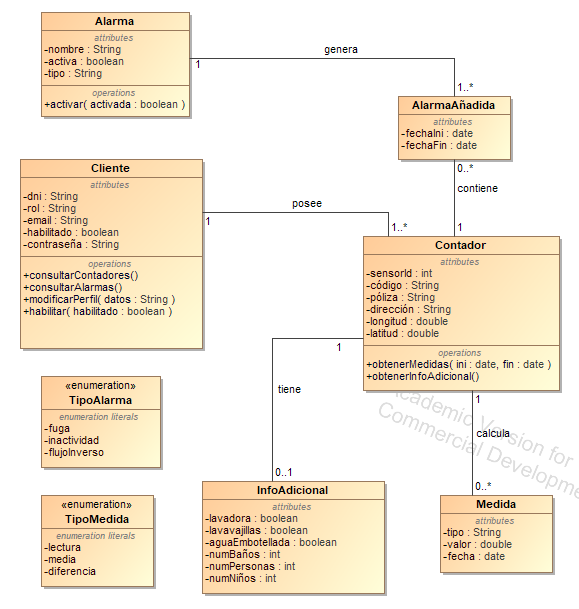
\includegraphics [scale=1] {images/diagramas/diagrama-clases.png}
 \caption{Diagrama de clases} \label{fig:diagrama-clases}
 \end{figure}


% ------------------------------------
\section{Diseño de la arquitectura del sistema}

Las aplicaciones web suelen basarse en el modelo Cliente/Servidor de tres capas, en el cual los clientes hacen peticiones al servidor web para obtener la información solicitada a través del protocolo \textit{HTTP} \cite{bib:arquitectura}. 

Las tres capas de este modelo son: la de presentación (parte del cliente y el servidor), la de proceso (servidor web) y de datos (servidor de datos) \cite{bib:arquitectura}. En la figura \ref{fig:arquitectura} se puede apreciar la arquitectura de la aplicación y la división entre sus capas.

 \begin{figure}[h]
 \centering
 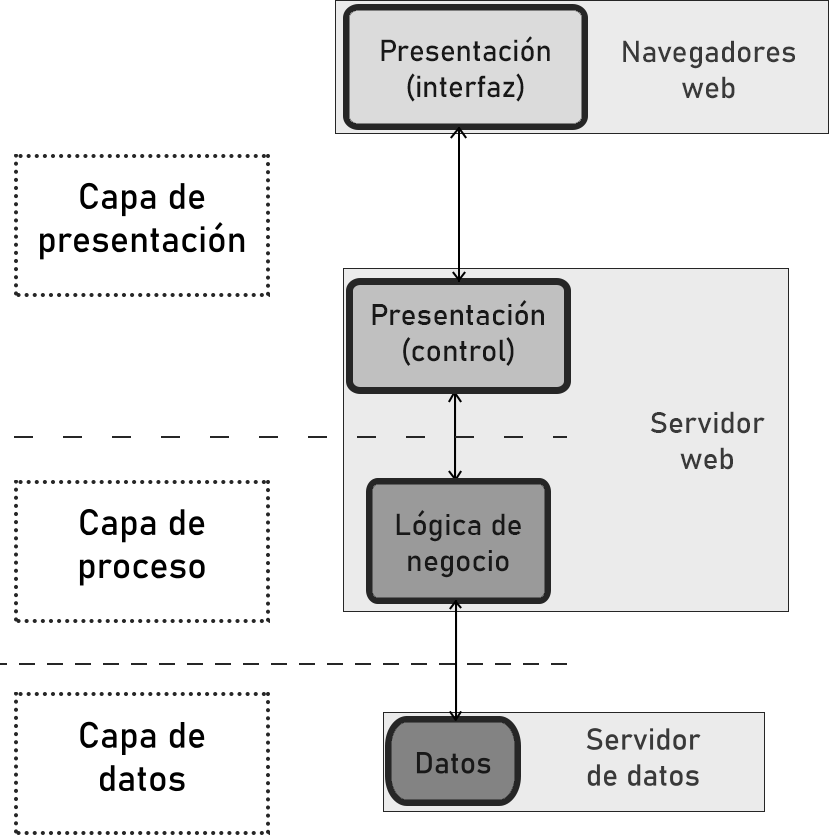
\includegraphics [scale=0.30] {images/diagramas/arquitectura.png}
 \caption{Esquema de la arquitectura} \label{fig:arquitectura}
 \end{figure}

\subsection{Base de datos}

Se creó una base de datos con el fin de almacenar la información personal de los usuarios y sus roles, así como los datos básicos de los contadores e información adicional de los mismos (véase figura \ref{fig:bbdd}). Por el contrario, no se creó ninguna tabla para el guardado de lecturas de los contadores ni alarmas. Esto se debió a que la administración de dichos datos la gestionaban varios microservicios que ya contaban con su propia base de datos. 


 \begin{figure}[H]
 \centering
 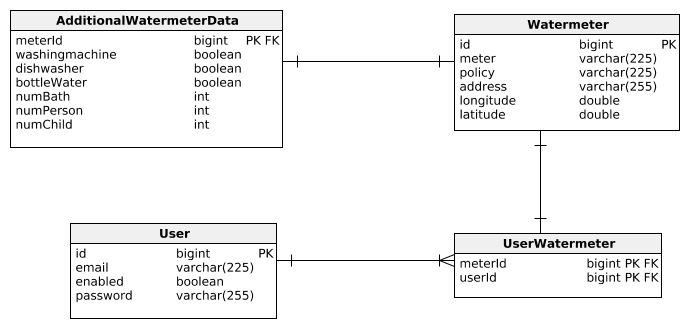
\includegraphics [scale=0.85] {images/diagramas/bbdd.png}
 \caption{Diseño lógico de la base de datos} \label{fig:bbdd}
 \end{figure}




% ------------------------------
\section{Diseño de la interfaz} \label{seccion:disenyo-interfaz}

Para el diseño de la interfaz de usuario, se partió del prototipo desarrollado por el mánager del equipo de desarrollo, el cual a su vez partió del diseño de una aplicación anteriormente implementada llamada \textit{Smart Water}. Esta aplicación está relacionada con la gestión de contadores, pero con la diferencia de estar enfocada únicamente al ámbito profesional, en concreto a las empresas que se dedican al abastecimiento de agua. Esto se explica con más detalle en la sección \ref{seccion:objetivos}.

También se tuvo en cuenta seguir las tres reglas de oro de Theo Mandel \cite{bib:3ReglasOro}, las cuales se citan a continuación:
\vspace{-4mm}
\begin{enumerate}
\addtolength{\itemsep}{-3mm}
\item Dar el control al usuario.
\item Reducir la carga de memoria del usuario.
\item Mantener la consistencia de la interfaz.
\end{enumerate}

La primera regla hace referencia a la libertad que tiene el usuario para interactuar con los elementos de la interfaz y deshacer o cancelar acciones \cite{bib:3ReglasOro}. La segunda se centra en hacer dicha interfaz lo más estructurada e intuitiva posible para que el usuario tenga que recordar la mínima información \cite{bib:3ReglasOro}.  La última regla trata de mantener la armonía visual en toda la aplicación para hacer predecible y cómoda la navegación por ella \cite{bib:3ReglasOro}.


% ---------------------------
\subsection{Definición de arquetipos y escenarios}

Sin embargo, para crear un diseño adecuado, no basta con tener en cuenta las tres reglas de oro anteriormente explicadas. Se debe conocer las características de los usuarios finales que usarán la aplicación para desarrollar un producto que se adecúe a ellos, teniendo en cuenta, su edad, sus costumbres, sus conocimientos, etc. A continuación, se explican dos arquetipos con dos escenarios distintos para cada uno, los cuales se definieron con la intención de tener una idea general de los tipos de usuarios finales que usarían la aplicación (véase tablas \ref{tablalarga:tablaArquetipo1} y \ref{tablalarga:tablaArquetipo2}). 


El primer arquetipo hace referencia a Marta Sánchez Ruiz, una posible cliente de esta aplicación a la que le gustaría consultar su consumo mensual de agua y programar alarmas para sus contadores con la intención de ser avisada en caso de haber alguna fuga o emergencia similar.

\vspace{5mm}

\textbf{Marta Sánchez Ruiz}
\vspace{-4mm}
\begin{itemize}
\addtolength{\itemsep}{-2mm}
\item [$-$] Mujer de mediana edad. 
\item [$-$] Usuaria frecuente de dispositivos informáticos como teléfonos móviles, \textit{tablets} y ordenadores.
\item [$-$] Accede a internet diariamente para ver periódicos digitales, ver vídeos en \textit{Youtube} o usar \textit{Netflix}.
\item [$-$] Eventualmente hace alguna compra \textit{online}.
\item [$-$] De vez en cuando accede de manera digital a su cuenta bancaria para comprobar gastos y recibos o hacer alguna transferencia.
\item [$-$] Pese a que está acostumbrada a hacer trámites por internet, no tiene una gran fluidez a la hora de llevarlos a cabo y de vez en cuando llega a pedir ayuda a algún familiar.
\item [$-$] Marta está registrada en la plataforma como cliente y ha iniciado sesión.
\end{itemize}

\vspace{5mm}

% -- Arquetipo Cliente ----
\renewcommand{\tablename}{Tabla}
\renewcommand{\arraystretch}{1,7}
\pretolerance=1000
\tolerance=1000

\begin{center}
\begin{longtable}{|m{3cm}|m{11cm}|}
\hline

\textbf{Escenario 1} & Marta desea consultar el consumo de agua de su casa este último mes y compararlo con el gasto promedio de su hogar, en el cual viven su pareja, sus dos hijos y ella. 
\\ \hline
Qué necesita & Espera que haya botón o pestaña visible y fácil de  reconocer para acceder al listado de sus contadores de agua, ya que tiene dos viviendas en propiedad. \break \break
Además, necesita que la información sobre el consumo del contador que esté consultando se vea de manera clara y comprensible. 
\\ \hline
\raggedright{Cómo le ayuda la \mbox{plataforma} web} &  La plataforma web debe contener un  listado de los contadores pertenecientes al cliente.  \break \break
La vista del contador consultado será fácil de entender gracias al diseño de la plataforma web, que mostrará la gráfica de consumo junto con un pequeño formulario para especificar el período de tiempo y la frecuencia que se quiere consultar.  \break \break
También dispondrá de datos del consumo del día actual, la diferencia con el día anterior y el promedio.  \break \break
A su vez habrá un pequeño listado con las alarmas que tiene el contador.
\\ \hline
\textbf{Escenario 2} & Marta desea activar una alarma para el contador de la casa de campo que tiene, la cual sólo visita en verano, para que le avise en caso de que se produzca una fuga.    
\\ \hline
Qué necesita & Espera que haya un botón o pestaña visible para poder programar una alarma en el contador en el que desea añadirla. \break \break
También necesita que el proceso sea fácil y rápido.
\\ \hline
\raggedright{Cómo le ayuda la \mbox{plataforma} web} & La plataforma web dispondrá de una pestaña en la cual se listen las alarmas de todos los contadores del cliente y un botón fácil de localizar llamado “Añadir”. \break \break
Además, se podrá añadir una alarma desde la vista que contiene la información de un contador, ya que en ésta también se verán las alarmas que contiene.
\\ \hline

\caption{Ejemplo de arquetipo de usuario cliente} \label{tablalarga:tablaArquetipo1}
\end{longtable}
\end{center}
% -----------------------
\vspace{-1,5cm}

El segundo arquetipo hace referencia a Sara Martínez García, una posible trabajadora de una empresa intermediaria entre la empresa encargada del suministro de agua de una zona y los clientes finales. Este tipo de empresa suele operar en una ciudad o pueblo concretos.

\vspace{5mm}
\textbf{Sara Martínez García}
\vspace{-4mm}
\begin{itemize}
\addtolength{\itemsep}{-2mm}
\item [$-$] Mujer de mediana edad.
\item [$-$] Oficinista.
\item [$-$] Usuaria común de dispositivos informáticos, especialmente del teléfono móvil y el ordenador, puesto que los utiliza durante su jornada laboral.
\item [$-$] Suele hacer trámites a través de internet.
\item [$-$] Accede a la plataforma desde su ordenador de oficina.
\item [$-$] Tiene una gran fluidez con el uso de diferentes programas y manejo del ordenador, ya que es fundamental para realizar su trabajo.
\item [$-$] Sara está registrada en la plataforma como administradora y ha iniciado sesión.
\end{itemize}

\vspace{5mm}

% ---- Arquetipo Administrador ---
\renewcommand{\tablename}{Tabla}
\renewcommand{\arraystretch}{1,7}
\pretolerance=1000
\tolerance=1000

\begin{center}
\begin{longtable}{|m{3cm}|m{11cm}|}
\hline

\textbf{Escenario 1} & Sara desea dar de alta a un nuevo cliente en la plataforma.
\\ \hline
Qué necesita & Espera poder realizar el alta del cliente de manera segura, con la opción de cancelar la operación en cualquier momento en caso de detectar algún error en los datos del cliente.
\\ \hline
\raggedright{Cómo le ayuda la \mbox{plataforma} web} & La plataforma web debe tener de una pestaña en la cual se listen los clientes que gestiona la administradora y un botón fácil de localizar llamado “Añadir nuevo cliente”. \break \break
También dispondrá de un formulario con los campos a rellenar el cual necesitará confirmación por parte de la administradora para poder registrar los datos proporcionados.
\\ \hline
\textbf{Escenario 2} & Sara desea consultar los datos del consumo promedio de los habitantes de una de las ciudades donde su empresa suministra el agua.    
\\ \hline
Qué necesita & Espera que haya algún tipo de filtro para poder indicar el listado de los contadores que desea ver.
Además, necesita poder ver el promedio de consumo de los contadores filtrados.
\\ \hline
\raggedright{Cómo le ayuda la \mbox{plataforma} web} & La plataforma web debe tener un listado de contadores con una serie de filtros, uno de ellos para indicar las localidades que se quieren consultar. \break \break
A su vez, se dispondrá de un campo de búsqueda donde poder escribir el nombre de un cliente para encontrar rápidamente sus contadores. \break \break
También tendrá un botón con el que poder calcular el promedio de consumo con los datos de los contadores filtrados.
\\ \hline
\caption{Ejemplo de arquetipo de usuario administrador} \label{tablalarga:tablaArquetipo2}
\end{longtable}
\end{center}
%-------------------------
\vspace{-1,5cm}

Como se puede observar en la tabla \ref{tablalarga:tablaArquetipo1}, el primer arquetipo hace referencia a un ciudadano de un municipio. En cambio, el segundo arquetipo está relacionado con el personal de una empresa intermediaria o ayuntamiento que administra las cuentas y da soporte a sus clientes. Los roles dentro de la plataforma de ambos arquetipos se han mencionado anteriormente al principio de la sección \ref{seccion:disenyo-interfaz}.


% -------------------------------

\subsection{Guía de estilos}

Los prototipos creados (véase anexo \ref{anexo:prototipos}) tienen en cuenta las pautas mencionadas anteriormente. El diseño es sencillo, con gráficas que facilitan la lectura al usuario y con paneles de información muy claros, concisos, sin textos largos y con iconos descriptivos.
Sin embargo, dichos prototipos no mostraban los colores y los estilos finales que se usaron en la implementación final (véase sección \ref{seccion:resultados-implementacion}), por lo que se diseñó una pequeña guía de estilo que los complementara. 

La paleta de colores que se utilizó en la interfaz de usuario, mostrada en la figura \ref{fig:paleta}, está compuesta principalmente por diferentes tonalidades de azul y gris. Esto fue debido a la intención de dar una sensación de tranquilidad y seriedad a la aplicación, así como relacionarla con la temática del agua y los contadores. Para llegar a esta conclusión se realizó un estudio previamente. Cabe añadir que la última fila hace referencia a los colores usados para mostrar avisos de errores, como sería la introducción de un campo inválido en un formulario.

\begin{figure}[H]
 \centering
 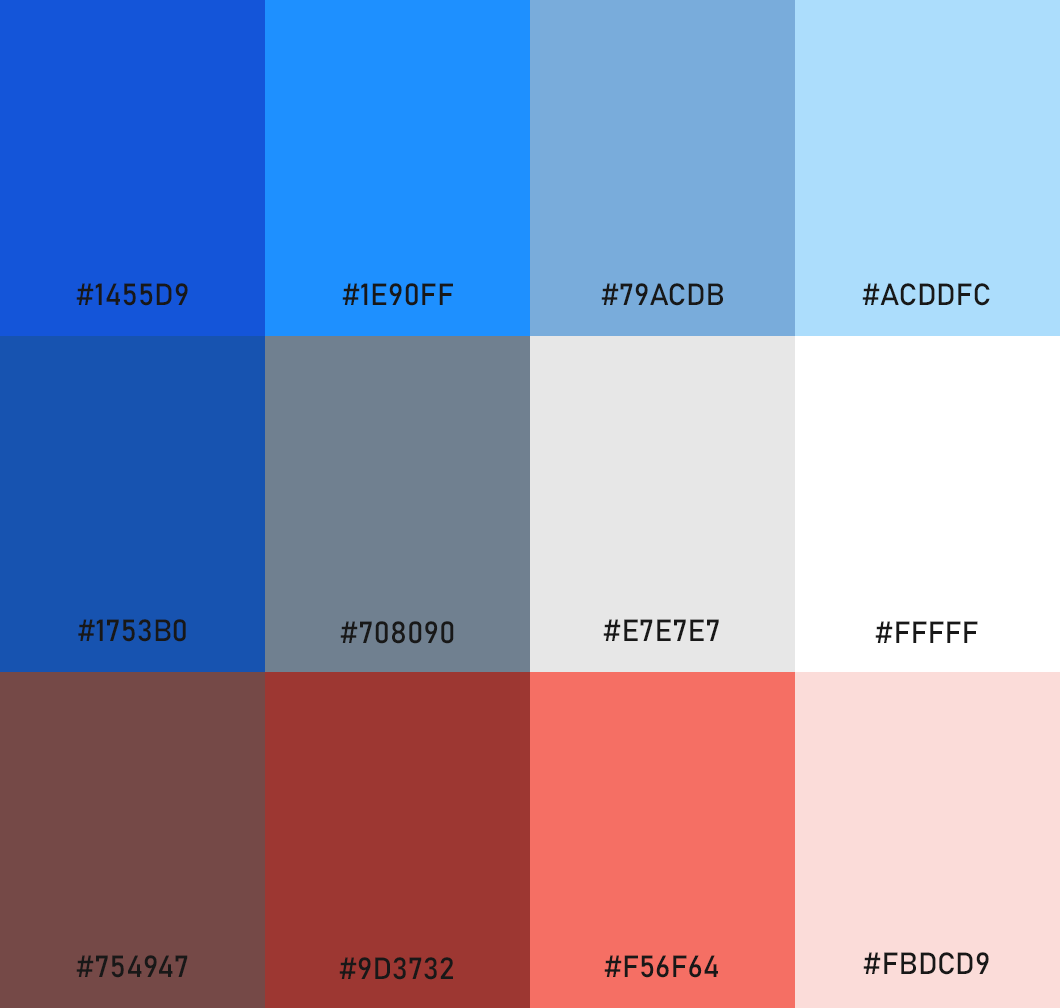
\includegraphics [scale=0.30] {images/disenyo/paleta-final.png}
 \caption{Paleta de colores} \label{fig:paleta}
 \end{figure}


Con respecto a los textos, para los encabezados y el cuerpo de cada vista, se establecieron unas directrices a seguir con la finalidad de ayudar a mantener la consistencia entre las diferentes vistas de la interfaz gráfica. Además, se optó por usar la fuente estándar \textit{Arial}, la cual es universalmente conocida y cómoda de leer. La tabla \ref{tablalarga:tablaTipografía} muestra el estilo y color establecidos para la tipografía según su función.

% ------ TABLA TIPOGRAFÍAS ----------
\renewcommand{\tablename}{Tabla}
\renewcommand{\arraystretch}{1,7}
\pretolerance=1000
\tolerance=1000

\begin{center}
\begin{longtable}{|>{\centering\arraybackslash}X m{5,5cm}|m{8,5cm}|}
\hline
\vspace{-5mm}
\includegraphics{images/disenyo/texto-h4.png} & Usada para indicar el título de cada bloque de información.
\\ \hline
\vspace{-4mm}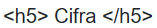
\includegraphics{images/disenyo/texto-h5.png} & Usada como texto informativo en los formularios y bloques con datos.
\\ \hline
\vspace{-4mm}
\includegraphics{images/disenyo/texto-p1.png} & Usada para los datos numéricos pertenecientes a las medidas tomadas del contador.
\\ \hline
\vspace{-4mm}
\includegraphics{images/disenyo/texto-p2.png} & Usada para las direcciones postales.

\\ \hline
\caption{Tipografías utilizadas en la interfaz gráfica} \label{tablalarga:tablaTipografía}
\end{longtable}
\end{center}
% -----------

\vspace{-1,5cm}

Por último, se diseñó el botón principal de la aplicación, el cual se utilizaría para las búsquedas, el guardado de datos y la autenticación del usuario. La tabla \ref{tablalarga:tablaBotón} que aparece a continuación muestra el diseño del botón en sus tres estados posibles.

% ------ TABLA BOTÓN ----------
\renewcommand{\tablename}{Tabla}
\renewcommand{\arraystretch}{1,7}
\pretolerance=1000
\tolerance=1000

\begin{center}
\begin{longtable}{|>{\centering\arraybackslash}X m{4cm}|>{\centering\arraybackslash}X m{4cm}|>{\centering\arraybackslash}X m{4cm}|}
\hline

\parbox[c]{\Includegraphics{images/disenyo/boton-normal.png}}  & 
\parbox[c]{\Includegraphics{images/disenyo/boton-seleccionado.png}} & 
\parbox[c]{\Includegraphics{images/disenyo/boton-deshabilitado.png}}
\\ \hline

Botón normal & Botón pulsado & Botón deshabilitado
\\ \hline

\caption{Diseño del botón principal} \label{tablalarga:tablaBotón}
\end{longtable}
\end{center}
% -----------------



%################## CAPÍTULO 4 - IMPLEMENTACIÓN  ############

\chapter{Implementación} \label{capitulo:implementacion}

% -----------------------
\section{Detalles de implementación}

La estructura general de la aplicación se muestra en la figura \ref{fig:estructura-general}. La parte del \textit{frontend} se implementó con el \textit{framework} de Angular, el cual se explica con más detenimiento en la sección \ref{seccion:tecnologia}. Además, se usaron varias librerías externas, como \textit{Transloco} para la traducción de los textos mostrados en la interfaz de usuario, \textit{Chart.js} para las gráficas, \textit{Leaflet} para la visualización de los mapas y \textit{Fortawsome-Angular} para los iconos.

 \begin{figure}[h]
 \centering
 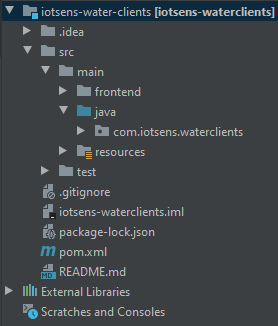
\includegraphics {images/implementacion/estructura-general.png}
 \caption{Estructura general de la aplicación} \label{fig:estructura-general}
 \end{figure}
 
 
Por el contrario, el directorio con el nombre de java contiene la parte del \textit{backend} de la aplicación. En su implementación se utilizó el \textit{framework} \textit{Spring}, definido con más detalle en la sección \ref{seccion:tecnologia}.

Por último, el directorio \textit{resources} contiene las sentencias de creación de la base de datos, así como varias inserciones por defecto con el fin de mantener una consistencia de datos mínima. Esto implica que si, por ejemplo, se borrara manualmente de la base de datos la tabla \textit{AdditionalWatermeterData} (véase figura \ref{fig:AdditionalWatermeterData.sql}), ésta se volvería a crear al ejecutarse la aplicación y añadiría los valores por defecto estipulados para cada contador. En caso de que los valores se fueran actualizando, esta sentencia no se ejecutaría, ya que no sería necesaria.

 \begin{figure}[h]
 \centering
 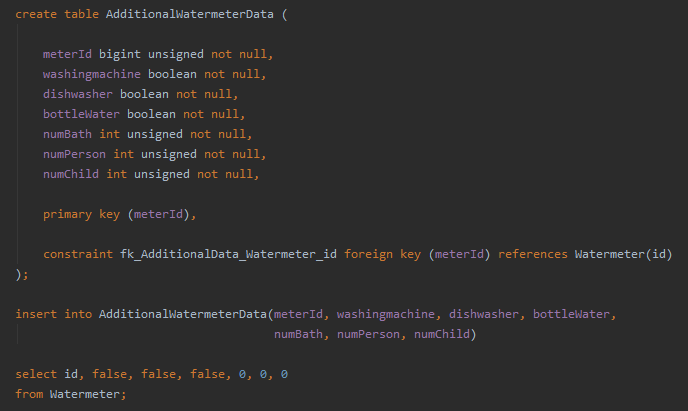
\includegraphics [scale=0.85] {images/implementacion/sentencia-sql.png}
 \caption{Fichero \textit{V5\_\_AdditionalWatermeterData.sql}} \label{fig:AdditionalWatermeterData.sql}
 \end{figure}

\vspace{1cm}
% ----------------

\subsection{Estructura del \textit{frontend}}

La estructura del \textit{frontend} de la aplicación está dividida principalmente en componentes, servicios y modelos. Antes de entrar en profundidad a explicarlos, se deben mencionar otros elementos que también la conforman.

Como se observa en la figura \ref{fig:estructura-frontend}, hay varios archivos de configuración situados en el directorio raíz del \textit{frontend} que contienen metadatos del proyecto, así como las dependencias que utiliza. Estos archivos van ligados con la carpeta \textit{nodes\_modules}, en la cual se encuentran las librerías instaladas. A su vez, se pueden visualizar los ficheros de inicio de la aplicación y el fichero \textit{styles.scss}. En este último se especifican los estilos comunes de la interfaz de usuario, como la tipografía, el color y forma de los botones, etc.

 \begin{figure}[H]
 \centering
 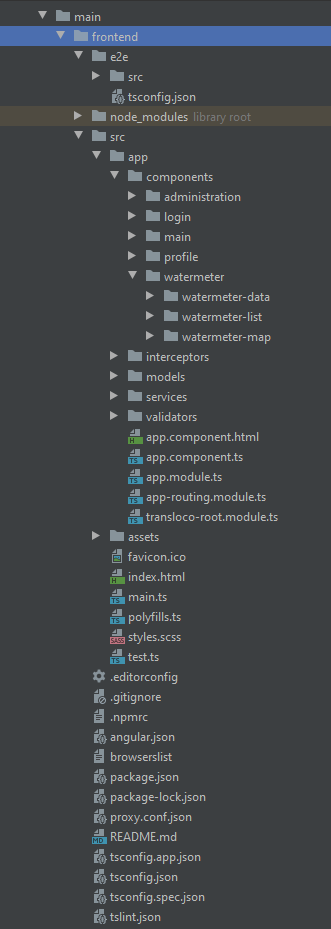
\includegraphics [scale=0.90] {images/implementacion/estructura-frontend.png}
 \caption{Estructura del \textit{frontend} de la aplicación} \label{fig:estructura-frontend}
 \end{figure}

Otro directorio que destacar es \textit{assets}, en que están almacenados los ficheros que contienen las traducciones de los textos que aparecen en las vistas. Para acceder a ellos se utiliza un servicio de la librería \textit{Transloco}, el cual se puede llamar tanto desde la vista como desde el controlador de un componente. Hay un ejemplo de su uso al principio del código mostrado en la figura \ref{fig:watermeter-html}.

 \begin{figure}[h]
 \centering
 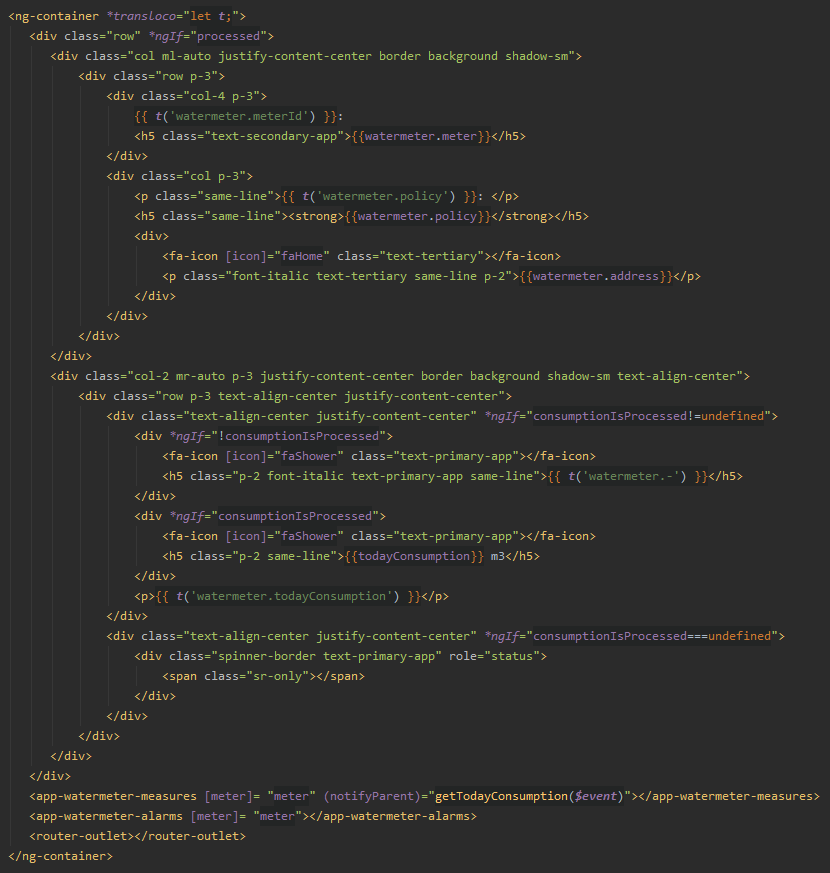
\includegraphics [scale=0.72] {images/implementacion/componente-watermeter-html.png}
 \caption{Código del fichero \textit{watermeter.component.html} (componente \textit{Watermeter})} \label{fig:watermeter-html}
 \end{figure}

Por otra parte, encontramos dentro del directorio \textit{app} los ficheros de enrutado de los componentes y su jerarquía. Esto es importante para poder especificar, por ejemplo, que la barra de navegación debe de estar presente en todas las vistas a excepción del \textit{Login}. Esta carpeta también contiene otros directorios, como \textit{validators}, que almacena los validadores usados para verificar los datos de los formularios, o \textit{interceptors}, para mostrar las vistas en función de los permisos que tengan los usuarios.

Con respecto a los componentes, cada uno de ellos está formado por dos ficheros. El primero (véase figura \ref{fig:watermeter-html}) es un fichero de \textit{html} que contiene únicamente lo elementos que se muestran al usuario y su formato, es decir, se trata de una vista completamente pasiva. El segundo fichero (véase \ref{fig:watermeter-ts}) tiene la extensión \textit{ts} y engloba el código que se encarga de pedir la información necesaria que debe mostrarse por pantalla. Este fichero contiene una clase de \textit{Typescript} con la anotación \textit{@Component}. A diferencia de otros \textit{frameworks} como \textit{React}, \textit{Angular} permite hacer este tipo de separación entre vista y controlador, facilitando así su implementación.

 \begin{figure}[h]
 \centering
 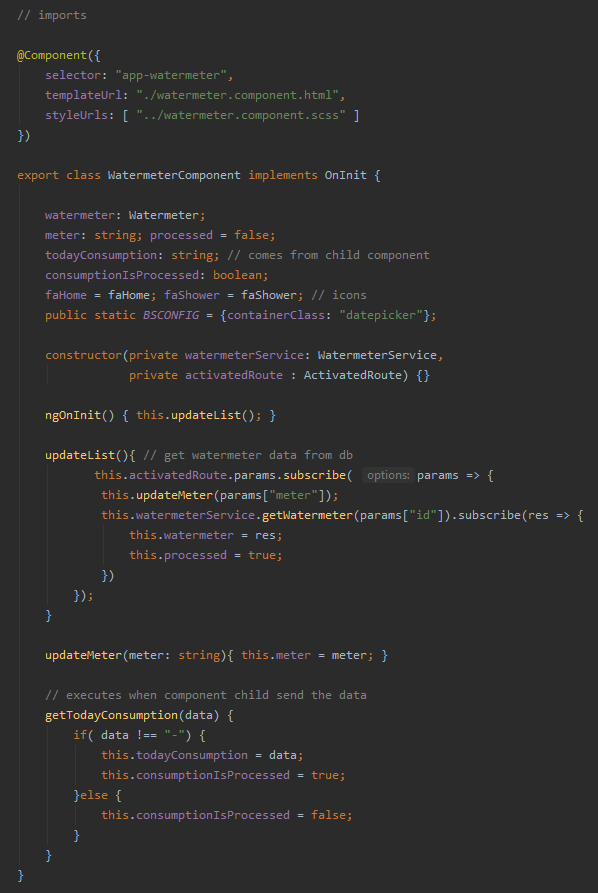
\includegraphics [scale=0.70] {images/implementacion/watermeter-ts.png}
 \caption{Código del fichero \textit{watermeter.component.ts} (componente \textit{Watermeter})} \label{fig:watermeter-ts}
 \end{figure}

Asimismo, se debe tener en cuenta que una determinada vista de la interfaz del usuario puede estar formada por varios componentes. En la aplicación, el componente que muestra una tabla con el listado de alarmas que tiene un contador lo engloba un componente padre que contiene los datos básicos de dicho contador y sus medidas. Al final del código mostrado en la \ref{fig:watermeter-html} se puede ver un ejemplo de ello, incluyendo el paso de parámetros y propiedades necesarios para que ambos componentes puedan comunicarse. 

Relacionado con esto último, se puede observar el mecanismo de comunicación entre el componente padre e hijos en la figura \ref{fig:measures-ts}, que hace referencia a un fragmento del componente hijo de \textit{Watermeter} y es el que muestra las lecturas del contador. El atributo que está marcado con la anotación \textit{@Input} sirve para obtener los valores de los parámetros pasados por el componente padre. Por el contrario, la anotación \textit{@Output} indica el evento que se ejecutará para avisar al componente padre y enviarle la información necesaria proveniente del hijo. Este tema está comentado en la subsección \ref{subseccion:desarrollo-implementacion}, el cual explica los problemas que hubo durante la implementación del \textit{frontend}.

 \begin{figure}[H]
 \centering
 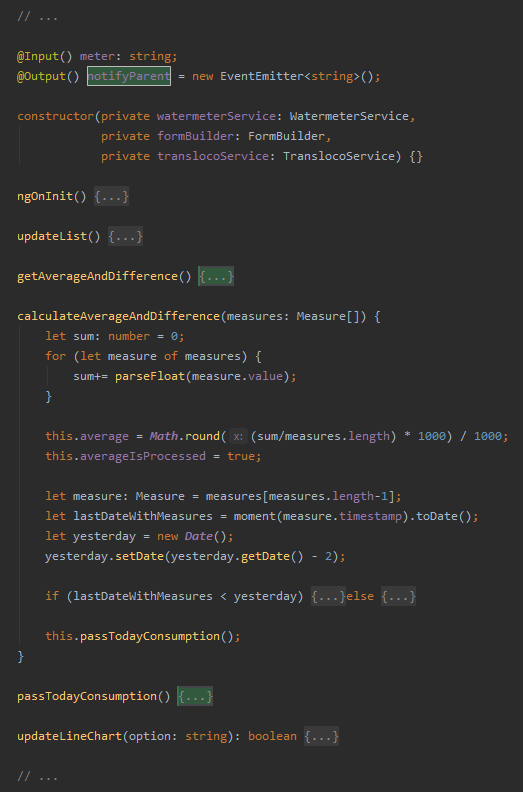
\includegraphics [scale=0.73] {images/implementacion/measures-ts.png}
 \caption{Fragmento del componente hijo de \textit{Watermeter} para obtener las lecturas del contador} \label{fig:measures-ts}
 \end{figure}



Otra característica a destacar de los componentes es la implementación de la interfaz \textit{OnInit} (véase figura \ref{fig:measures-ts}), que sirve para indicar qué métodos se quieren ejecutar al renderizar la vista del componente. También se debe considerar cómo realiza la llamada al método de un servicio, ya que realmente se suscribe a él para ser notificado cuando le lleguen los datos y, mientras tanto, se ejecute paralelamente el resto del programa. Esto es así para optimizar su ejecución, ya que si se quiere hacer más de una consulta a la base de datos sería tedioso tener que esperar a que acabaran todas ellas para cargar la vista. En otras palabras, los servicios implementan el patrón \textit{Observer} a través del uso de los \textit{observables} de \textit{Angular}. Además, como se muestra en la \ref{fig:watermeter-html}, es posible indicar cuándo se debe visualizar determinados elementos de la vista usando \textit{*ngIf}, puesto que consulta una variable booleana que cambia una vez se reciben los datos. 


Por otro lado, están los servicios, que son los que se comunican directamente con el \textit{backend} de la aplicación y en ellos están definidas las llamadas necesarias para tal propósito. Pueden ser utilizados por diferentes componentes y cada servicio se encarga de la gestión de un determinado tipo de datos, como las medidas de un contador, las alarmas o la información del usuario. La figura \ref{fig:service-watermeter} hace referencia un fragmento de la clase \textit{watermeter.service.ts}, en el cual se puede ver los dos tipos de llamadas: la que realiza para obtener la información adicional de un contador y la que actualiza los datos. Como se puede observar, no es necesario indicar la \textit{URL}\footnote{Localizador Uniforme de Recursos o \textit{Uniform Resource Identifier} en inglés. Hace referencia a la dirección específica de un recurso red con el fin de poder identificarlo \cite{bib:url}} del \textit{backend} completa, ésta se puede especificar en los ficheros de configuración.

 \begin{figure}[h]
 \centering
 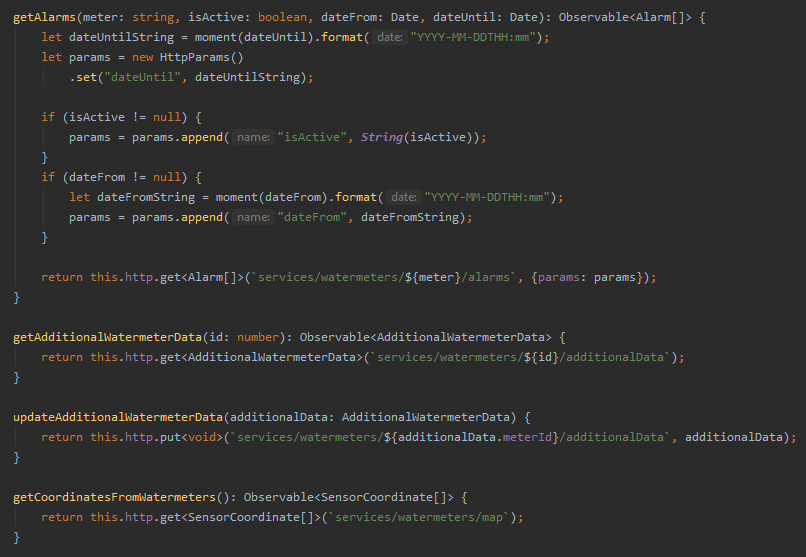
\includegraphics [scale=0.73] {images/implementacion/service-watermeter.png}
 \caption{Fragmento del fichero \textit{watermeter.service.ts}} \label{fig:service-watermeter}
 \end{figure}

En referencia a los modelos, éstos son clases en \textit{Typscript} que ayudan a dar forma a los datos provenientes del \textit{backend}. La figura \ref{fig:model-watermeter} muestra la clase \textit{Watermeter.ts}, correspondiente a los datos básicos que tiene un contador. Para que la información se almacene correctamente, es necesario que la clase tenga los mismos atributos y se llamen igual que las clases definidas en el modelo del \textit{backend} (véase figura \ref{fig:model-watermeter-java}).


 \begin{figure}[h]
 \centering
 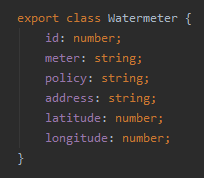
\includegraphics [scale=0.72] {images/implementacion/watermeter-model.png}
 \caption{Clase \textit{Watermeter.ts}} \label{fig:model-watermeter}
 \end{figure}
 

Finalmente, cabe destacar el uso del patrón MVVM (\textit{model-view-viewmodel}) en la implementación del \textit{frontend}, el cual es una variación del patrón clásico MVC (modelo-vista-controlador, o en inglés \textit{model-view-controller}). Esto es así debido a la sincronización de datos que tiene el \textit{framework Angular}, el cual implica una dependencia entre la vista y el modelo \cite{bib:angular-MVC}.


%------------------------

\subsection{Estructura del \textit{backend}}

La estructura del \textit{backend} de la aplicación se puede contemplar en la figura \ref{fig:estructura-backend}, que muestra una serie de directorios entre los que podemos encontrar \textit{services} y \textit{models}, los cuales tienen el mismo nombre que en el \textit{frontend} (véase figura \ref{fig:estructura-frontend}). Ambos desempeñan funciones similares, aunque en este caso los servicios son más bien los intermediarios que hacen consultas a microservicios externos o usan los métodos de las clases que se encargan de pedir la información a la base de datos. Los servicios también están divididos según sus cometidos, son usados por los controladores y están marcados con la anotación \textit{@Service}.

Por el contrario, los modelos, al igual que en \textit{frontend}, sirven para representar los datos obtenidos de las peticiones de la base de datos y los microservicios.

\begin{figure}[H]
 \centering
 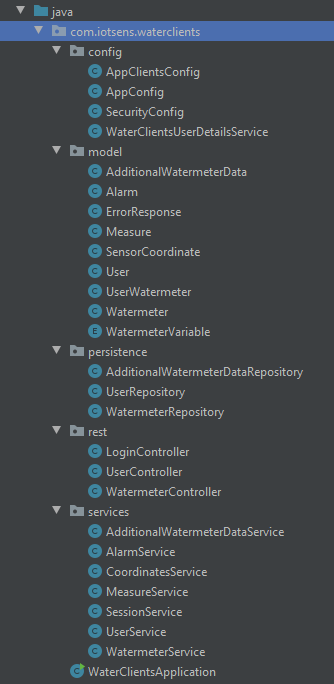
\includegraphics [scale=1] {images/implementacion/estructura-backend.png}
 \caption{Estructura del \textit{backend} de la aplicación} \label{fig:estructura-backend}
 \end{figure}


Si estos datos provienen de las consultas de la base de datos, requieren de un método estático que genere un objeto de esa clase (véase figura \ref{fig:model-watermeter-java}). Además, su tratamiento y transformación se realizan en las clases que se encuentran en el directorio \textit{persistence}. Estas clases están marcadas con la anotación \textit{@Repository} y son las popularmente conocidas como DAOs (Objeto de Acceso a Datos, en inglés \textit{Data Acess Object}), ya que implementan este patrón de diseño. Parte de la implementación de una de ellas se puede examinar en la figura \ref{fig:watermeter-repository}. 


 \begin{figure}[H]
 \centering
 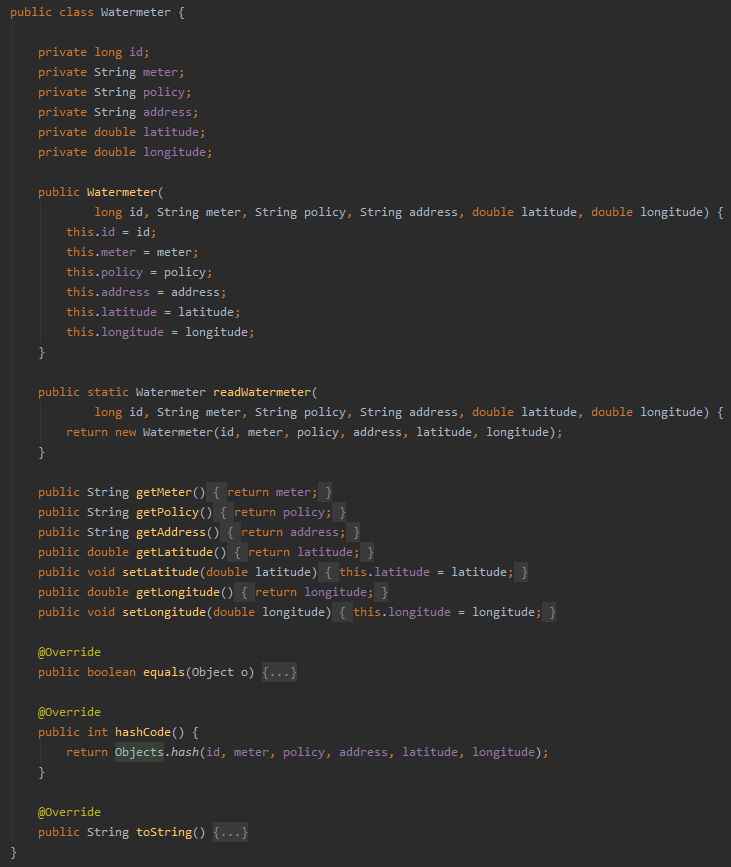
\includegraphics [scale=0.85] {images/implementacion/watermeter-model-java.png}
 \caption{Clase \textit{Watermeter.java}} \label{fig:model-watermeter-java}
 \end{figure}
 

 \begin{figure}[H]
 \centering
 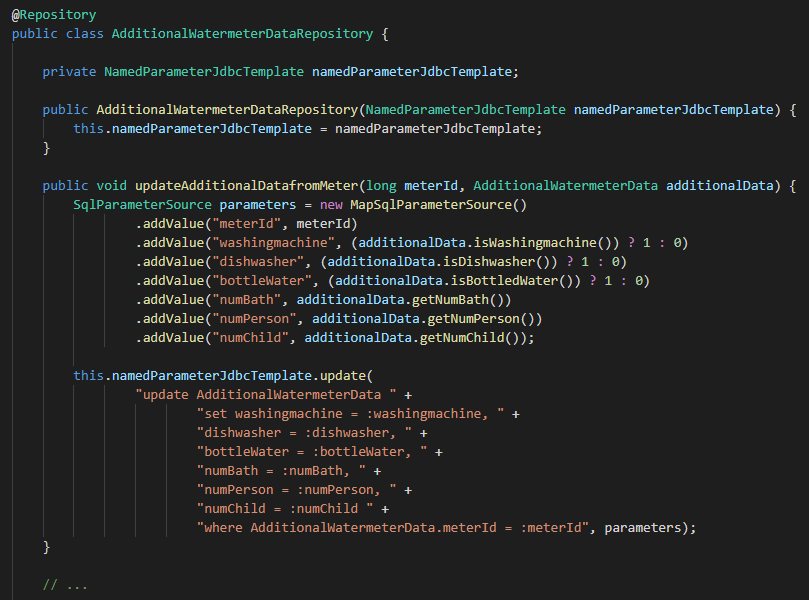
\includegraphics [scale=0.72] {images/implementacion/watermeter-repository.png}
 \caption{Fragmento de la clase \textit{AdditionalWatermeterDataRepository.java}} \label{fig:watermeter-repository}
 \end{figure}

Por otro lado, en el directorio \textit{rest} se encuentra la implementación los controladores que mapean las peticiones \textit{http} al \textit{backend} de la aplicación. Estas clases están señaladas con la anotación \textit{@RestController} que proporciona el \textit{framework Spring} y contienen los servicios que van a utilizar. A su vez, estas clases utilizan otras anotaciones como \textit{@RequestMapping} para indicar la ruta común o \textit{@GetMapping} para especificar que es una petición de tipo \textit{GET}. La figura \ref{fig:watermeter-controller} muestra un fragmento de la clase \textit{WatermerController.java} donde se observa la estructura de estos controladores. 

Al describir estos elementos que conforman la estructura del \textit{backend}, es posible percatarse de la presencia del patrón compuesto \textit{MVC}. El \textit{framework Spring} facilita su implementación gracias a sus anotaciones, clases y métodos propios. 

 \begin{figure}[H]
 \centering
 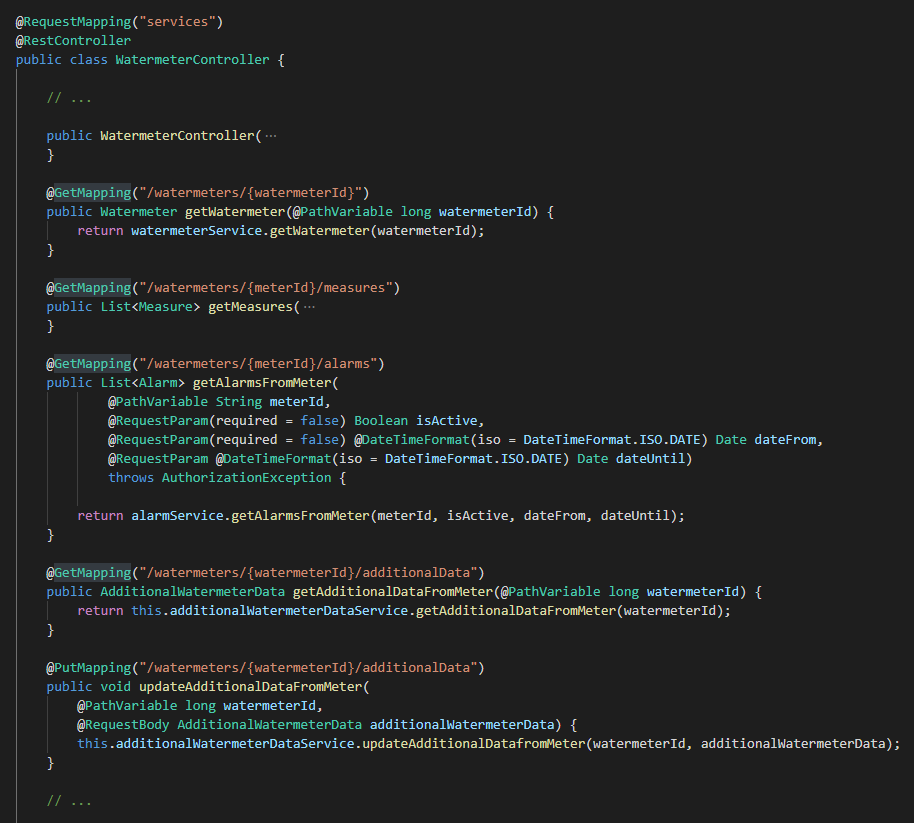
\includegraphics [scale=0.65] {images/implementacion/watermeter-controller.png}
 \caption{Fragmento de la clase \textit{WatermeterController.java}} \label{fig:watermeter-controller}
 \end{figure}


Finalmente, se debe mencionar el directorio \textit{config} que, como su nombre indica, contiene las configuraciones globales del \textit{backend} de la aplicación, así como las restricciones de seguridad, el acceso a la base de datos y a los microservicios.  La configuración de acceso a estas últimas está representada en la figura \ref{fig:watermeter-config}. En ella se puede comprobar cómo se obtienen las credenciales necesarias a través de la anotación \textit{@Value} con el fin de acceder a los microservicios utilizados para la obtención de medidas y alarmas de los contadores. También se puede observar cómo se crea una instancia de esos microservicios con la anotación \textit{@Bean}, que hace uso del patrón \textit{Singleton}. 


 \begin{figure}[H]
 \centering
 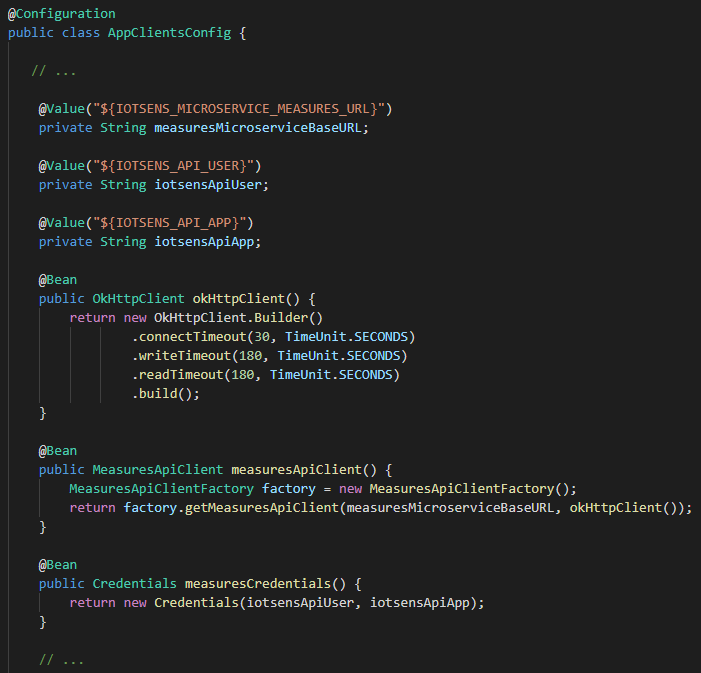
\includegraphics [scale=0.65] {images/implementacion/watermeter-config.png}
 \caption{Fragmento de la clase \textit{AppiClientsConfig.java}} \label{fig:watermeter-config}
 \end{figure}
 
 \subsection{Desarrollo de la implementación} \label{subseccion:desarrollo-implementacion}
 
 Entre los problemas que surgieron durante la implementación del \textit{frontend}, el más destacable fue el paso de información entre componentes. Esto se debió a que, en algunos casos, se debía estimar si valía la pena crear una dependencia entre componente padre e hijo o hacer varias peticiones al \textit{backend}. En el caso de los componentes que mostraban las alarmas y las medidas de un contador, se optó por obtener los datos necesarios desde el componente padre, el cual contenía la información básica de dicho contador. Se llegó a esa conclusión por el hecho de estar fuertemente relacionados entre sí, ya que todos ellos formaban parte de una única vista en la interfaz de usuario.
También se tomó la decisión de no calcular el consumo promedio total de todos los contadores del cliente al no ser un dato útil que consultar, a diferencia de lo que se mostraba en el prototipo inicial (véase figura \ref{fig:prototipo6} del anexo \ref{anexo:prototipos}).

Durante el desarrollo del \textit{backend}se optó por hacer uso de las expresiones lambda para simplificar la transformación de datos. Esto estuvo ligado a la decisión de hacer las llamadas a los microservicios directamente en los propios servicios del \textit{backend}, sin necesidad de utilizar ninguna clase intermediaria encargada de gestionarlas. Esto se debió a una cuestión de simplicidad, ya que sólo se requería llamar a los métodos del microservicio instanciado y construir el resultado obtenido mediante una expresión lambda sencilla. La figura \ref{fig:watermeter-service-java} representa la implementación de la clase \textit{AlarmService}. 

\begin{figure}[H]
 \centering
 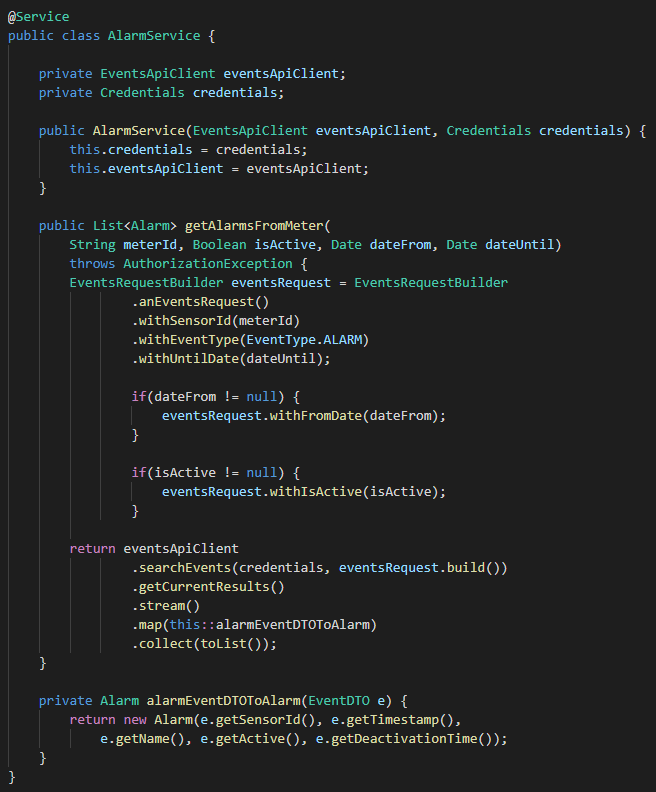
\includegraphics [scale=0.90] {images/implementacion/watermeter-service-java.png}
 \caption{Clase \textit{AlarmService.java}} \label{fig:watermeter-service-java}
 \end{figure}

%------------------------------------------------

\section{Resultados de la implementación} \label{seccion:resultados-implementacion}

A continuación, se muestran los resultados de la implementación realizada durante la estancia de prácticas. Esto engloba tanto las funcionalidades implementadas de la aplicación como la apariencia final de cada componente, los cuales están presentados desde la figura \ref{fig:vista-login} hasta la figura \ref{fig:vista-datos-adicionales}. Cabe mencionar que todas las vistas y operaciones mostradas hacen referencia a las del cliente, puesto que las del administrador las desarrolló otro miembro del equipo. En la sección \ref{seccion:seguimiento-proyecto} se explica con más detalle la planificación y la división de tareas. 

\subsection{Vista del \textit{login}} \label{subseccion:vista-login}

La figura \ref{fig:vista-login} presenta la vista del \textit{login} de la aplicación. Comparado con el resto de las vistas, en ella no se muestra la barra de navegación, ya que necesitas acceder a la aplicación primero.

\begin{figure}[h]
 \centering
 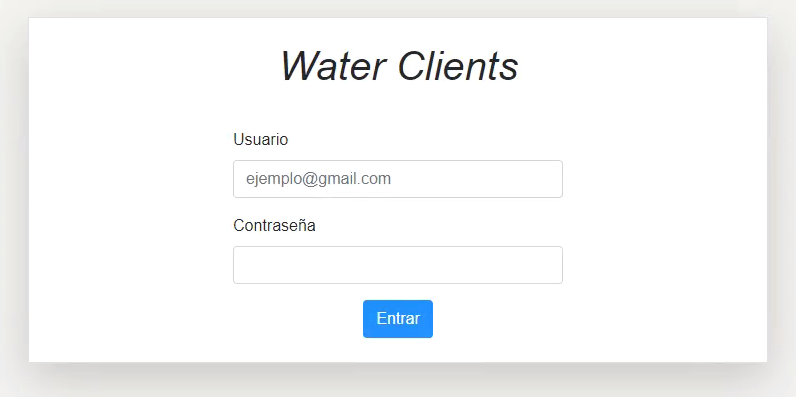
\includegraphics [scale=0.75] {images/vistas/login.png}
 \caption{Vista del \textit{login}} \label{fig:vista-login}
 \end{figure}

\subsection{Vista del listado de contadores} \label{subseccion:vista-listado}

La figura \ref{fig:vista-lista-contadores}  muestra un fragmento del listado de contadores que componen la vista. Como se puede apreciar, tanto en esta vista como en las siguientes se observa la barra de navegación. Esto se debe a la jerarquía establecida en los ficheros de configuración del \textit{frontend} para los componentes que conforman las vistas.

\begin{figure}[H]
 \centering
 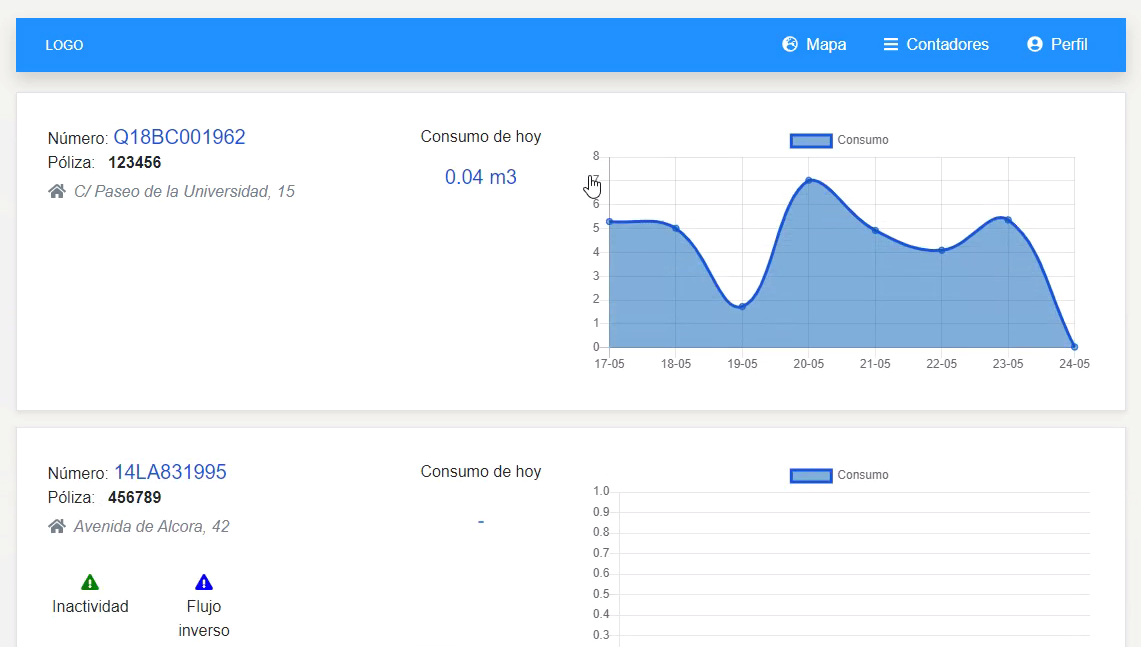
\includegraphics [scale=0.52] {images/vistas/listado-contadores.png}
 \caption{Vista del listado de contadores del usuario} \label{fig:vista-lista-contadores}
 \end{figure}

\subsection{Vista del contador} \label{subseccion:vista-contador}

La vista completa del contador lo componen una serie de figuras divididas en los diferentes componentes que la conforman. Las figuras \ref{fig:vista-contador} , \ref{fig:vista-lecturas} y \ref{fig:vista-alarmas} muestran de manera ordenada la vista completa.


\begin{figure}[h]
 \centering
 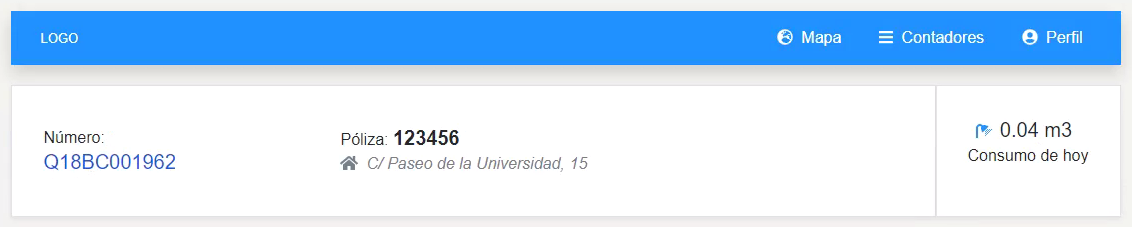
\includegraphics [scale=0.53] {images/vistas/contador.png}
 \caption{Componente con los datos básicos del contador (Vista del contador)} \label{fig:vista-contador}
 \end{figure}
 
 \begin{figure}[H]
 \centering
 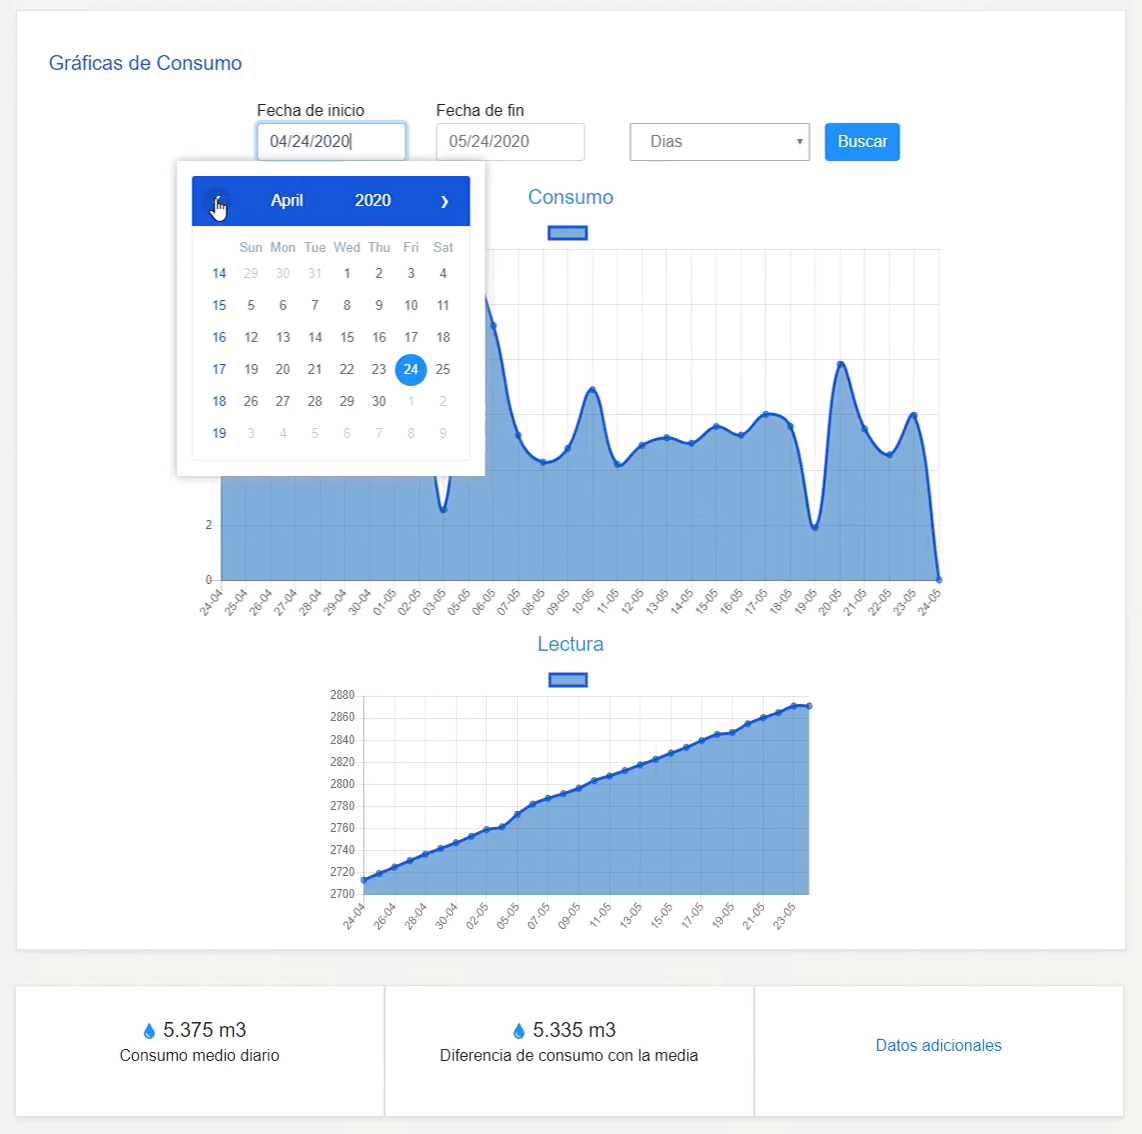
\includegraphics [scale=0.39] {images/vistas/lecturas-componentes.png}
 \caption{Componente con las lecturas del contador (Vista del contador)} \label{fig:vista-lecturas}
 \end{figure}

 \begin{figure}[H]
 \centering
 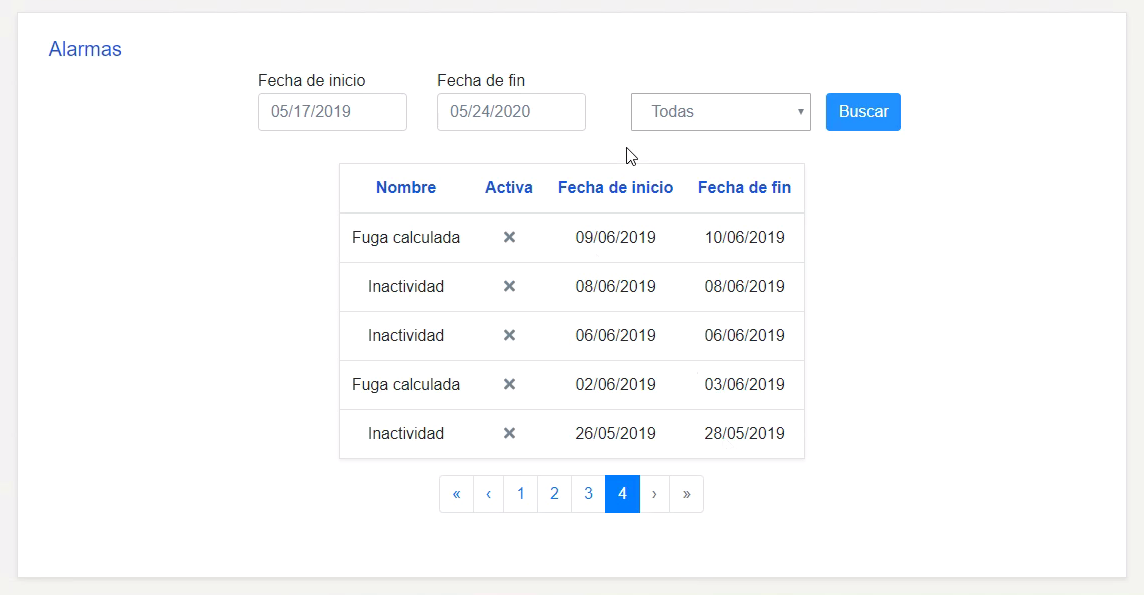
\includegraphics [scale=0.50] {images/vistas/alarmas.png}
 \caption{Componente con las alarmas del contador (Vista del contador)} \label{fig:vista-alarmas}
 \end{figure}
% -----------------------

\subsection{Vista del mapa}

 La figura \ref{fig:vista-mapa} muestra la vista del mapa que contiene las ubicaciones de los contadores de un usuario, los cuales están representados con marcadores que muestran la información básica del contador cuando se seleccionan. 

 \begin{figure}[h]
 \centering
 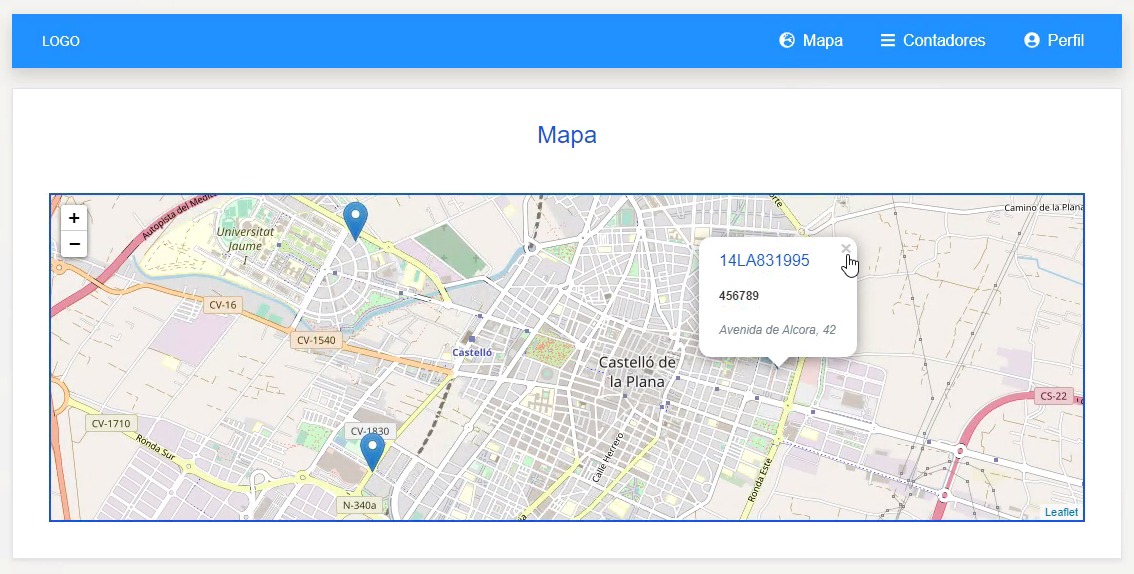
\includegraphics [scale=0.53] {images/vistas/mapa.png}
 \caption{Vista del mapa con los marcadores de los contadores del usuario} \label{fig:vista-mapa}
 \end{figure}
 % -----------------------
 
 \subsection{Vista de la información adicional}
 
 Como se puede observar en la figura \ref{fig:vista-datos-adicionales}, la vista que muestra la información adicional de un contador es un formulario. Esto es debido a la comodidad de poder modificar en cualquier momento los datos, lo que también proporciona una libertad y flexibilidad al usuario para poder cancelar la operación en cualquier momento. Por otro lado, esta vista al igual que la del mapa, está conformada por un único componente.

 \begin{figure}[h]
 \centering
 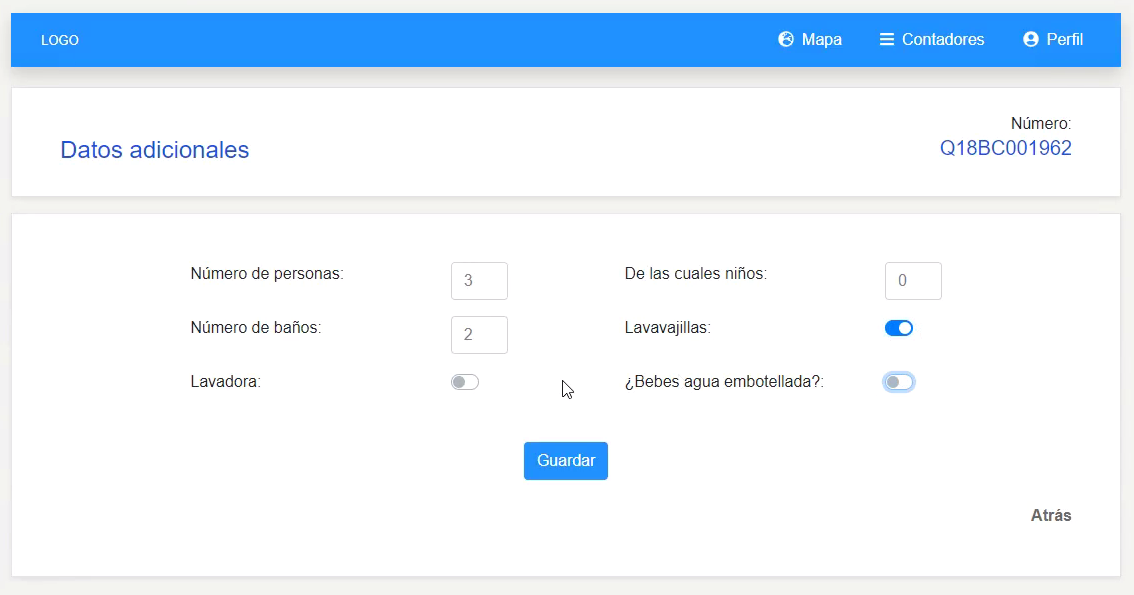
\includegraphics [scale=0.53] {images/vistas/datos-adicionales.png}
 \caption{Vista del formulario con los datos adicionales de un contador} \label{fig:vista-datos-adicionales}
 \end{figure}













%################ CAPÍTULO 5 - PRUEBAS ############

\chapter{Verificación y validación} \label{capitulo:verificacion-validacion}

\section{Pruebas de aceptación} \label{seccion:pruebas-aceptacion}

Una parte fundamental en el desarrollo de un proyecto informático de calidad es el \textit{testing}.  Éste nos permite comprobar que la aplicación realice correctamente las funciones para las que ha sido desarrollada y que contenga la mínima cantidad de \textit{bugs} o fallos. Normalmente, las empresas suelen contar con un departamento de QA (\textit{Quality Aassurance}) y/o \textit{testers} que ayudan a cumplir este propósito. 

Existen muchos tipos de pruebas con el fin de garantizar la calidad del producto \textit{software}. Para este proyecto se definieron una serie de pruebas de aceptación, compuestas cada una por un escenario válido e inválido, creadas a partir de las historias de usuario contenidas en la pila del producto (véase tabla \ref{tablalarga:tablaHU}). Este tipo de pruebas van dirigidas tanto a usuarios como desarrolladores, para poder tener una visión general del comportamiento de la aplicación. Las tablas de la \ref{tablalarga:tablaPA01} a la \ref{tablalarga:tablaPA07} muestran las pruebas de aceptación creadas para probar las funcionalidades desarrolladas durante la estancia en prácticas. 


% ---------- TABLA PA01 --------------

\renewcommand{\tablename}{Tabla}
\renewcommand{\arraystretch}{1,7}
\pretolerance=1000
\tolerance=1000

\begin{center}
\begin{longtable}{|>{\centering\arraybackslash}X m{2cm}|m{12cm}|}
\hline
\multicolumn{2}{|c|}{\textbf{Prueba de aceptación PA01}}\\
\hline 
\endhead

\textbf{Historia de usuario} & Como usuario quiero loguearme en la plataforma para poder consultar la información de mis contadores de agua y mi consumo.
\\ \hline

\textbf{Escenario válido} & {\raggedright El usuario tiene conexión con la base de datos.\par}
\vspace{2mm}
\break

\underline{Given}:
\begin{itemize}
\addtolength{\itemsep}{-3mm}
\item Email: \textit{cliente123@gmail.com}
\item Contraseña: \textit{password321}
\end{itemize}
\vspace{3mm}

\underline{When}:
\begin{enumerate}
\vspace{-3mm}
\addtolength{\itemsep}{-3mm}
\item El usuario solicita acceder a la aplicación.
\item La aplicación hace una petición a la base de datos del cliente con el email \textit{cliente123@gmail.com}.
\item El sistema verifica la contraseña.
\end{enumerate}
\break

\underline{Then}:
\vspace{-3mm}
\begin{itemize}
\addtolength{\itemsep}{-3mm}
\item \underline{Salida esperada}: se muestra la página principal de la aplicación.
\item \underline{Estado esperado}: se crea y almacena el token del usuario.
\end{itemize}


\\ \hline
\textbf{Escenario inválido} & {\raggedright El usuario tiene conexión con la base de datos.\par}
\vspace{2mm}
\break

\underline{Given}:
\vspace{-3mm}
\begin{itemize}
\addtolength{\itemsep}{-3mm}
\item Email: \textit{cliente123@gmail.com}
\item Contraseña: \textit{pkyefgeyb}
\end{itemize}

\underline{When}:
\begin{enumerate}
\vspace{-3mm}
\addtolength{\itemsep}{-3mm}
\item El usuario solicita acceder a la aplicación.
\item La aplicación hace una petición a la base de datos del cliente con el email \textit{cliente123@gmail.com}.
\item El sistema invalida la contraseña.
\end{enumerate}
\break

\underline{Then}:
\vspace{-3mm}
\begin{itemize}
\addtolength{\itemsep}{-3mm}
\item \underline{Salida esperada}: se muestra la página principal de la aplicación.
\item \underline{Estado esperado}: se crea y almacena el token del usuario.
\end{itemize}
\\ \hline

\caption{Prueba de aceptación PA01.} \label{tablalarga:tablaPA01}
\end{longtable}
\end{center}
% --------------------------------

% ----- TABLA PA02 -----------

\renewcommand{\tablename}{Tabla}
\renewcommand{\arraystretch}{1,7}
\pretolerance=1000
\tolerance=1000

\begin{center}
\begin{longtable}{|>{\centering\arraybackslash}X m{2cm}|m{12cm}|}
\hline
\multicolumn{2}{|c|}{\textbf{Prueba de aceptación PA02}}\\
\hline 
\endhead

\textbf{Historia de usuario} & Como usuario quiero ver mi lista de contadores para saber sus datos.
\\ \hline

% --- VÁLIDO
\textbf{Escenario válido} & El usuario está logueado, tiene conexión con la base de datos y los microservicios que gestionan las alarmas y las lecturas.
\vspace{2mm}
\break

\underline{Given}:
\begin{itemize}
\addtolength{\itemsep}{-3mm}
\item Token del usuario: \textit{7163jwk452}
\item Id del usuario: \textit{1533}
\end{itemize}
\vspace{3mm}

\underline{When}:
\begin{enumerate}
\vspace{-3mm}
\addtolength{\itemsep}{-3mm}
\item El usuario solicita ver el listado de contadores.
\item El sistema verifica el token del usuario.
\item La aplicación hace una petición a la base de datos.
\item La aplicación hace una petición al microservicio que gestiona las alarmas.
\item La aplicación hace una petición al microservicio que gestiona las lecturas.
\end{enumerate}
\break

\underline{Then}:
\vspace{-3mm}
\begin{itemize}
\addtolength{\itemsep}{-3mm}
\item \underline{Salida esperada}:  se muestra un listado con los datos de cada contador junto con el consumo del día, una pequeña gráfica y los iconos de las alarmas activas.
\item \underline{Estado esperado}: no se almacena ninguna información.
\end{itemize}

% --- INVÁLIDO
\\ \hline
\textbf{Escenario inválido} & {\raggedright El usuario está logueado, tiene conexión con la base de datos pero no con los microservicios.\par}
\vspace{2mm}
\break

\underline{Given}:
\vspace{-3mm}
\begin{itemize}
\addtolength{\itemsep}{-3mm}
\item Token del usuario: \textit{7163jwk452}
\item Id del usuario: \textit{1533}
\end{itemize}

\underline{When}:
\begin{enumerate}
\vspace{-3mm}
\addtolength{\itemsep}{-3mm}
\item El usuario solicita ver el listado de contadores.
\item El sistema verifica el token del usuario.
\item La aplicación hace una petición a la base de datos.
\item La aplicación hace una petición al microservicio que gestiona las alarmas.
\item La aplicación hace una petición al microservicio que gestiona las lecturas.
\end{enumerate}
\break

\underline{Then}:
\vspace{-3mm}
\begin{itemize}
\addtolength{\itemsep}{-3mm}
\item \underline{Salida esperada}: se muestra un listado con los datos básicos de cada contador, no se muestran las alarmas y se indica con un guión que no se ha podido obtener la lectura.
\item \underline{Estado esperado}: no se almacena ninguna información.
\end{itemize}
\\ \hline

\caption{Prueba de aceptación PA02.} \label{tablalarga:tablaPA02}
\end{longtable}
\end{center}

% ----------------------

% ---------- TABLA PA03 --------------

\renewcommand{\tablename}{Tabla}
\renewcommand{\arraystretch}{1,7}
\pretolerance=1000
\tolerance=1000

\begin{center}
\begin{longtable}{|>{\centering\arraybackslash}X m{2cm}|m{12cm}|}
\hline
\multicolumn{2}{|c|}{\textbf{Prueba de aceptación PA03}}\\
\hline 
\endhead

\textbf{Historia de usuario} & Como usuario quiero consultar la información de un contador para saber los datos del contador.

\\ \hline

\textbf{Escenario válido} & {\raggedright El usuario está logueado y tiene conexión con la base de datos.\par}
\vspace{2mm}
\break

\underline{Given}:
\begin{itemize}
\addtolength{\itemsep}{-3mm}
\item Token del usuario: \textit{7163jwk452}
\item Id del usuario: \textit{1533}
\item Id del contador: \textit{Q7629UY760}
\end{itemize}
\vspace{3mm}

\underline{When}:
\begin{enumerate}
\vspace{-3mm}
\addtolength{\itemsep}{-3mm}
\item El usuario solicita ver la información de un contador.
\item El sistema verifica el token del usuario.
\item La aplicación hace una petición a la base de datos.
\end{enumerate}
\break

\underline{Then}:
\vspace{-3mm}
\begin{itemize}
\addtolength{\itemsep}{-3mm}
\item \underline{Salida esperada}: confirmación de la petición, se muestra por pantalla el identificador, la póliza y la dirección del contador \textit{Q7629UY760}.
\item \underline{Estado esperado}: no se almacena ninguna información en una base de datos.
\end{itemize}

% -- inválido
\\ \hline
\textbf{Escenario inválido} & {\raggedright El usuario está logueado pero no tiene conexión con la base de datos.\par}
\vspace{2mm}
\break

\underline{Given}:
\vspace{-3mm}
\begin{itemize}
\addtolength{\itemsep}{-3mm}
\item Token del usuario: \textit{7163jwk452}
\item Id del usuario: \textit{1533}
\item Id del contador: \textit{Q7629UY760}
\end{itemize}

\underline{When}:
\begin{enumerate}
\vspace{-3mm}
\addtolength{\itemsep}{-3mm}
\item El usuario solicita ver la información de un contador.
\item El sistema verifica el token del usuario.
\item La aplicación intenta conectarse a la base de datos sin éxito.
\end{enumerate}
\break

\underline{Then}:
\vspace{-3mm}
\begin{itemize}
\addtolength{\itemsep}{-3mm}
\item \underline{Salida esperada}: se muestra por pantalla el mensaje de error “En estos momentos no es posible mostrar la información, por favor inténtelo más tarde”.
\item \underline{Estado esperado}: no se guarda ningún dato.
\end{itemize}
\\ \hline

\caption{Prueba de aceptación PA03.} \label{tablalarga:tablaPA03}
\end{longtable}
\end{center}

% -----------------------


% ---------- TABLA PA04 --------------

\renewcommand{\tablename}{Tabla}
\renewcommand{\arraystretch}{1,7}
\pretolerance=1000
\tolerance=1000

\begin{center}
\begin{longtable}{|>{\centering\arraybackslash}X m{2cm}|m{12cm}|}
\hline
\multicolumn{2}{|c|}{\textbf{Prueba de aceptación PA04}}\\
\hline 
\endhead

\textbf{Historia de usuario} & Historia de usuario	Como usuario quiero elegir el período de tiempo para visualizar de manera gráfica el gasto de agua que indica un contador.

\\ \hline

\textbf{Escenario válido} & {\raggedright El usuario está logueado y tiene conexión con la base de datos y al microservicio que gestiona las lecturas.\par}
\vspace{2mm}
\break

\underline{Given}:
\begin{itemize}
\addtolength{\itemsep}{-3mm}
\item Token del usuario: \textit{7163jwk452}
\item Id del usuario: \textit{1533}
\item Id del contador: \textit{Q7629UY760}
\item Fecha inicio: \textit{02/03/2020}
\item Fecha fin: \textit{24/05/2020}
\item Intervalo: \textit{semanas}

\end{itemize}
\vspace{3mm}

\underline{When}:
\begin{enumerate}
\vspace{-3mm}
\addtolength{\itemsep}{-3mm}
\item El usuario solicita saber el consumo realizado entre el día \textit{02/03/2020} y \textit{24/05/2020}, en intervalos de semanas.
\item El sistema verifica el período de tiempo dado.
\item El sistema verifica el token del usuario.
\item La aplicación hace una petición a la base de datos. 
\item La aplicación hace una petición al microservicio que gestiona las lecturas.
\end{enumerate}
\break

\underline{Then}:
\vspace{-3mm}
\begin{itemize}
\addtolength{\itemsep}{-3mm}
\item \underline{Salida esperada}: confirmación de la petición, se actualiza la gráfica mostrada por pantalla con los datos nuevos.
\item \underline{Estado esperado}: no se almacena ninguna información en una base de datos.
\end{itemize}

% --- inválido --- 
\\ \hline
\textbf{Escenario inválido} & {\raggedright El usuario está logueado, tiene conexión con la base de datos y al microservicio que gestiona las lecturas.\par}
\vspace{2mm}
\break

\underline{Given}:
\vspace{-3mm}
\begin{itemize}
\addtolength{\itemsep}{-3mm}
\item Token del usuario: \textit{7163jwk452}
\item Id del usuario: \textit{1533}
\item Id del contador: \textit{Q7629UY760}
\item Fecha inicio: \textit{09/12/2021}
\item Fecha fin: \textit{15/07/2019}
\item Intervalo: \textit{semanas}

\end{itemize}

\underline{When}:
\begin{enumerate}
\vspace{-3mm}
\addtolength{\itemsep}{-3mm}
\item El usuario solicita saber el consumo realizado del período incorrecto entre el \textit{09/12/2021} y \textit{15/07/2019}, en intervalos de semanas.
\item El sistema invalida el periodo de tiempo dado.

\end{enumerate}
\break

\underline{Then}:
\vspace{-3mm}
\begin{itemize}
\addtolength{\itemsep}{-3mm}
\item \underline{Salida esperada}: se indica por pantalla el mensaje de error “Período de tiempo inválido”.
\item \underline{Estado esperado}: no se actualizan los datos.
\end{itemize}
\\ \hline

\caption{Prueba de aceptación PA04.} \label{tablalarga:tablaPA04}
\end{longtable}
\end{center}
% -------------------------

\newpage
% ---------- TABLA PA05 --------------

\renewcommand{\tablename}{Tabla}
\renewcommand{\arraystretch}{1,7}
\pretolerance=1000
\tolerance=1000

\begin{center}
\begin{longtable}{|>{\centering\arraybackslash}X m{2cm}|m{12cm}|}
\hline
\multicolumn{2}{|c|}{\textbf{Prueba de aceptación PA05}}\\
\hline 
\endhead

\textbf{Historia de usuario} & Como usuario quiero visualizar las alarmas programadas de un contador en un período de tiempo para saber cuáles tengo activas y cuáles no.

\\ \hline

\textbf{Escenario válido} & {\raggedright El usuario está logueado, tiene conexión con la base de datos y al microservicio que gestiona las alarmas.\par}
\vspace{2mm}
\break

\underline{Given}:
\begin{itemize}
\addtolength{\itemsep}{-3mm}
\item Token del usuario: \textit{7163jwk452}
\item Id del usuario: \textit{1533}
\item Id del contador: \textit{Q7629UY760}
\item Fecha inicio: \textit{02/03/2020}
\item Fecha fin: \textit{24/05/2020}
\item Alarmas: \textit{todas}

\end{itemize}
\vspace{3mm}

\underline{When}:
\begin{enumerate}
\vspace{-3mm}
\addtolength{\itemsep}{-3mm}
\item El usuario solicita saber todas las alarmas (activas e inactivas) de un contador entre el día \textit{02/03/2020} y \textit{24/05/2020}.
\item El sistema verifica el período de tiempo dado.
\item El sistema verifica el token del usuario.
\item La aplicación hace una petición a la base de datos.  
\item La aplicación hace una petición al microservicio que gestiona las alarmas.

\end{enumerate}
\break

\underline{Then}:
\vspace{-3mm}
\begin{itemize}
\addtolength{\itemsep}{-3mm}
\item \underline{Salida esperada}: confirmación de la petición, se actualiza la tabla mostrada por pantalla con los datos nuevos.
\item \underline{Estado esperado}: no se almacena ninguna información en una base de datos.
\end{itemize}

% --- Inválido ---
\\ \hline
\textbf{Escenario inválido} & {\raggedright El usuario está logueado, tiene conexión con la base de datos pero no al microservicio que gestiona las alarmas.

\par}
\vspace{2mm}
\break

\underline{Given}:
\vspace{-3mm}
\begin{itemize}
\addtolength{\itemsep}{-3mm}
\item Token del usuario: \textit{7163jwk452}
\item Id del usuario: \textit{1533}
\item Id del contador: \textit{Q7629UY760}
\item Fecha inicio: \textit{02/03/2020}
\item Fecha fin: \textit{24/05/2020}
\item Alarmas: \textit{activas}

\end{itemize}

\underline{When}:
\begin{enumerate}
\vspace{-3mm}
\addtolength{\itemsep}{-3mm}
\item El usuario solicita saber las alarmas activas de un contador entre el día \textit{02/03/2020} y \textit{24/05/2020}.
\item El sistema verifica el período de tiempo dado.
\item El sistema verifica el token del usuario.
\item La aplicación hace una petición a la base de datos. 
\item La aplicación intenta conectarse al microservicio que gestiona las alarmas sin éxito.

\end{enumerate}
\break

\underline{Then}:
\vspace{-3mm}
\begin{itemize}
\addtolength{\itemsep}{-3mm}
\item \underline{Salida esperada}: se indica por pantalla el mensaje de error “No se han podido mostrar las alarmas del contador”.
\item \underline{Estado esperado}: no se actualizan los datos.
\end{itemize}
\\ \hline

\caption{Prueba de aceptación PA05.} \label{tablalarga:tablaPA05}
\end{longtable}
\end{center}
% ------------------------------------


% ---------- TABLA PA06 --------------

\renewcommand{\tablename}{Tabla}
\renewcommand{\arraystretch}{1,7}
\pretolerance=1000
\tolerance=1000

\begin{center}
\begin{longtable}{|>{\centering\arraybackslash}X m{2cm}|m{12cm}|}
\hline
\multicolumn{2}{|c|}{\textbf{Prueba de aceptación PA06}}\\
\hline 
\endhead

\textbf{Historia de usuario} & Como usuario quiero rellenar un formulario con información adicional de un contador para poder especificar mejor las condiciones que se deberían de tener en cuenta a la hora de mostrar datos estadísticos y predictivos de mi consumo de agua.

\\ \hline

\textbf{Escenario válido} & {\raggedright El usuario está logueado y tiene conexión con la base de datos.\par}
\vspace{2mm}
\break

\underline{Given}:
\begin{itemize}
\addtolength{\itemsep}{-3mm}
\item Token del usuario: \textit{7163jwk452}
\item Id del usuario: \textit{1533}
\item Id del contador: \textit{Q7629UY760}
\item Cantidad de personas: \textit{4}
\item Cantidad de baños: \textit{2}
\item Lavavajillas: \textit{no}

\end{itemize}
\vspace{3mm}

\underline{When}:
\begin{enumerate}
\vspace{-3mm}
\addtolength{\itemsep}{-3mm}
\item El usuario solicita actualizar los datos adicionales relativos al contador \textit{Q7629UY760}.
\item El sistema confirma que no hay errores en el formulario.
\item El sistema verifica el token del usuario.
\item La aplicación intenta conectarse a la base de datos sin éxito.

\end{enumerate}
\break

\underline{Then}:
\vspace{-3mm}
\begin{itemize}
\addtolength{\itemsep}{-3mm}
\item \underline{Salida esperada}: confirmación de la petición, se actualizan los datos mostrados.
\item \underline{Estado esperado}: almacena la información en la base de datos y se actualizan los datos anteriores.
\end{itemize}

% --- inválidos ---
\\ \hline
\textbf{Escenario inválido} & {\raggedright El usuario está logueado y tiene conexión con la base de datos.\par}
\vspace{2mm}
\break

\underline{Given}:
\vspace{-3mm}
\begin{itemize}
\addtolength{\itemsep}{-3mm}
\item Token del usuario: \textit{7163jwk452}
\item Id del usuario: \textit{1533}
\item Id del contador: \textit{Q7629UY760}
\item Cantidad de personas: \textit{-56}
\item Cantidad de baños: \textit{sthsd}
\item Lavavajillas: \textit{no}

\end{itemize}

\underline{When}:
\begin{enumerate}
\vspace{-3mm}
\addtolength{\itemsep}{-3mm}
\item El usuario solicita actualizar los datos adicionales incorrectos relativos al contador \textit{Q7629UY760}.
\item El sistema indica que hay errores en el formulario.

\end{enumerate}
\break

\underline{Then}:
\vspace{-3mm}
\begin{itemize}
\addtolength{\itemsep}{-3mm}
\item \underline{Salida esperada}: se indica por pantalla que los campos de personas y baños son inválidos.
\item \underline{Estado esperado}: no se almacena ninguna información en la base de datos y no se actualizan los datos anteriores.
\end{itemize}
\\ \hline

\caption{Prueba de aceptación PA06.} \label{tablalarga:tablaPA06}
\end{longtable}
\end{center}
% ------------------------

% ---------- TABLA PA07 --------------

\renewcommand{\tablename}{Tabla}
\renewcommand{\arraystretch}{1,7}
\pretolerance=1000
\tolerance=1000

\begin{center}
\begin{longtable}{|>{\centering\arraybackslash}X m{2cm}|m{12cm}|}
\hline
\multicolumn{2}{|c|}{\textbf{Prueba de aceptación PA07}}\\
\hline 
\endhead

\textbf{Historia de usuario} & Como usuario quiero consultar en un mapa la posición de mis contadores para así poder visualizar su ubicación geográfica.
\\ \hline

\textbf{Escenario válido} & {\raggedright El usuario está logueado y tiene conexión con la base de datos.\par}
\vspace{2mm}
\break

\underline{Given}:
\begin{itemize}
\addtolength{\itemsep}{-3mm}
\item Token del usuario: \textit{7163jwk452}
\item Id del usuario: \textit{1533}

\end{itemize}
\vspace{3mm}

\underline{When}:
\begin{enumerate}
\vspace{-3mm}
\addtolength{\itemsep}{-3mm}
\item El usuario solicita ver la ubicación de sus contadores.
\item El sistema verifica el token del usuario.
\item La aplicación hace una petición a la base de datos.

\end{enumerate}
\break

\underline{Then}:
\vspace{-3mm}
\begin{itemize}
\addtolength{\itemsep}{-3mm}
\item \underline{Salida esperada}: confirmación de la petición, se muestra por pantalla la ubicación del contador \textit{Q7629UY760}.
\item \underline{Estado esperado}: no se almacena ninguna información en una base de datos.
\end{itemize}


\\ \hline
\textbf{Escenario inválido} & {\raggedright El usuario está logueado pero no tiene conexión con la base de datos.\par}
\vspace{2mm}
\break

\underline{Given}:
\vspace{-3mm}
\begin{itemize}
\addtolength{\itemsep}{-3mm}
\item oken del usuario: \textit{7163jwk452}
\item Id del usuario: \textit{1533}

\end{itemize}

\underline{When}:
\begin{enumerate}
\vspace{-3mm}
\addtolength{\itemsep}{-3mm}
\item El usuario solicita ver la ubicación de sus contadores.
\item El sistema verifica el token del usuario.
\item La aplicación intenta conectarse a la base de datos sin éxito.

\end{enumerate}
\break

\underline{Then}:
\vspace{-3mm}
\begin{itemize}
\addtolength{\itemsep}{-3mm}
\item \underline{Salida esperada}: se muestra por pantalla el mapa sin ningún marcador y el mensaje de error “En estos momentos no es posible mostrar la ubicación de los sensores, por favor inténtelo más tarde”.
\item \underline{Estado esperado}: no se almacena ninguna información en una base de datos.
\end{itemize}
\\ \hline

\caption{Prueba de aceptación PA07.} \label{tablalarga:tablaPA07}
\end{longtable}
\end{center}

% --------------- FINAL DE TABLAS PA -----------


% -------------------------

\section{Pruebas unitarias y de integración} \label{seccion:pruebas-unitarias-integracion}

A nivel de \textit{backend}, un miembro del grupo se encargó de realizar tanto pruebas unitarias como de integración. Con respecto a las primeras, se implementaron test unitarios para comprobar el correcto funcionamiento de métodos y clases de manera aislada. Puesto que algunos de estos métodos y clases tenían dependencias externas, como la base de datos y los microservicios, se usó un \textit{mock}\footnote{Son objetos preprogramados que simulan el comportamiento de objetos reales y se usan para probar y verificar el correcto funcionamiento de las llamadas a otros métodos \cite{bib:mock}.} llamado \textit{Mokito}, que imitaba el comportamiento de estas dependencias. 


Una vez hechas estas primeras comprobaciones, se procedió a analizar la interacción entre el software y su entorno real, es decir, se examinó su funcionamiento con la base de datos y los microservicios. Esta tarea la llevó a cabo el mánager del proyecto, encargado de supervisar que todas las funcionalidades implementadas por cada miembro del equipo quedaran correctamente integradas en la aplicación.


Con respecto al \textit{frontend}, tanto Google como otros navegadores web disponen de herramientas para los desarrolladores. Con la finalidad de verificar el envío de datos y las consultas \textit{HTTP} al \textit{backend}, se utilizó el inspector de \textit{Google Chorme} y la aplicación \textit{Advanced REST client}. Esta extensión, pese a ser más simple que la aplicación de \textit{Postman}, permitía hacer comprobaciones rápidas de las consultas al \textit{backend} e informar de los errores producidos o de si se había realizado con éxito la operación. La figura \ref{fig:pruebas} muestra el error 404 al proporcionarle una id incorrecta de un contador para obtener sus lecturas.

 \begin{figure}[h]
 \centering
 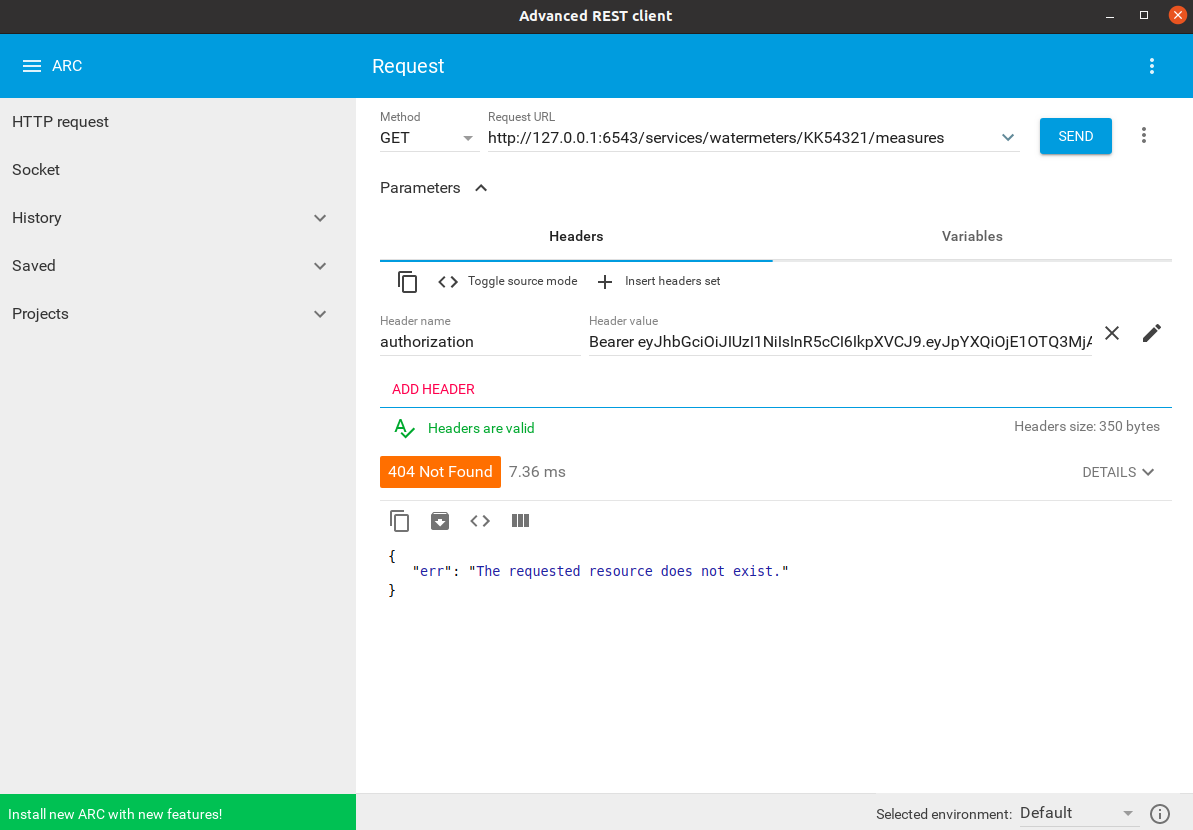
\includegraphics [scale=0.35] {images/implementacion/pruebas.png}
 \caption{Ejemplo de petición fallida usando la aplicación \textit{Advanced REST client}} 
 \label{fig:pruebas}
 \end{figure}



% ---------------------------




%################# CAPÍTULO 6 - CONCLUSIONES ###################

\chapter{Conclusiones} \label{capitulo:conclusiones}

La realización de este proyecto ha sido una experiencia enriquecedora en varios aspectos. En primer lugar, he adquirido conocimientos de tecnologías con las que todavía no había trabajado, como el \textit{framework Angular} y el lenguaje de programación \textit{Typescript}. 

También he tenido la oportunidad de vivir de primera mano el proceso que sigue la empresa IoTsens desde que genera la propuesta técnica de un producto \textit{software} para un cliente, hasta que se empieza a implementar.

En lo que respecta a la experiencia laboral, trabajar y coordinarse con un equipo profesional en circunstancias adversas ha mejorado, sin duda alguna, mis capacidades de adaptación a situaciones inesperadas. Esto es especialmente importante por el hecho de haber realizado la mitad de mi estancia de prácticas de remotamente, ya que la pandemia del COVID-19 obligó a tener que permanecer en casa.

Por otro lado, me hubiera gustado tener la oportunidad de aplicar los conocimientos de \textit{machine learning}, adquiridos durante la última semana de prácticas, a la aplicación. Desgraciadamente, esto no fue posible debido a que faltaban funcionalidades que implementar de mayor prioridad. Además, la parte de \textit{machine learning} se consideró en todo momento una mejora del producto original. No obstante, el resultado final obtenido ha sido bueno y se han completado los objetivos esperados durante el período de estancia en prácticas.

Finalmente quería destacar que, en general, he aprendido mucho de esta experiencia y me ha ayudado a conseguir recientemente un puesto de trabajo como \textit{IT Engineer} en el departamento de desarrollo de una empresa belga. Mi adaptación e integración en este nuevo entorno de trabajo y equipo ha sido rápida gracias a la experiencia adquirida durante las prácticas, a pesar de utilizar otras tecnologías.






% ########## BIBLIOGRAFÍA #############


%\bibliography{bibliografia.bib}

\cleardoublepage
\phantomsection
\addcontentsline{toc}{chapter}{Bibliografía}
\bibliography{bibliografia.bib}
\bibliographystyle{plain}



% ------------------- Anexos ---------------------

\appendix
\renewcommand\appendixname{Anexo}



% ---- Primer Anexo ----
\chapter{Prototipos de la aplicación} \label{anexo:prototipos-aplicacion}

\section{Prototipos de las vistas del cliente} \label{anexo:prototipos}

\begin{figure}[h]
 \centering
 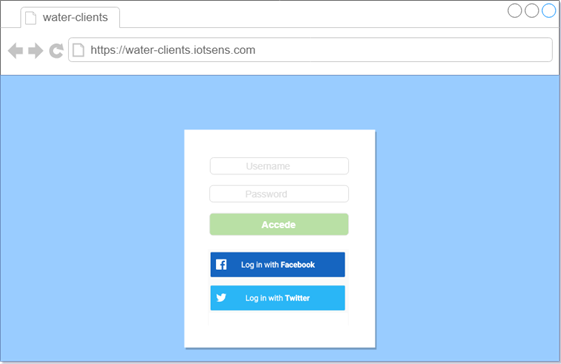
\includegraphics [scale=1] {images/prototipo/imagen1.png}
 \caption{Prototipo del \textit{login} de la aplicación} \label{fig:prototipo1}
 \end{figure}
 
 \begin{figure}[h]
 \centering
 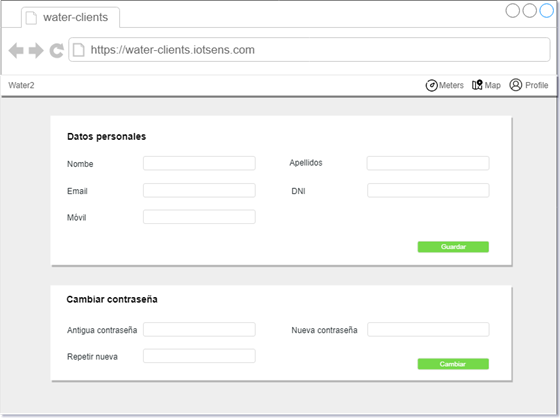
\includegraphics [scale=1] {images/prototipo/imagen2.png}
 \caption{Prototipo del panel del perfil de usuario} \label{fig:prototipo2}
 \end{figure}
 
 \begin{figure}[h]
 \centering
 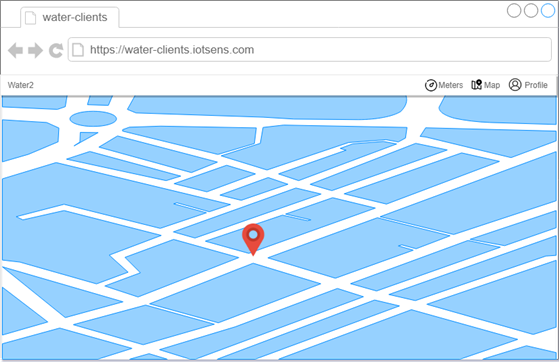
\includegraphics [scale=1] {images/prototipo/imagen3.png}
 \caption{Prototipo del mapa con la localización de los contadores} \label{fig:prototipo3}
 \end{figure}
 
 \begin{figure}[h]
 \centering
 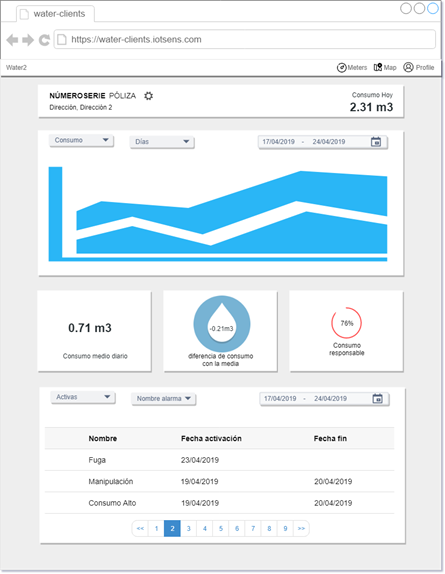
\includegraphics [scale=1] {images/prototipo/imagen4.png}
 \caption{Prototipo del panel de datos y alarmas del contador} \label{fig:prototipo4}
 \end{figure}

 \begin{figure}[h]
 \centering
 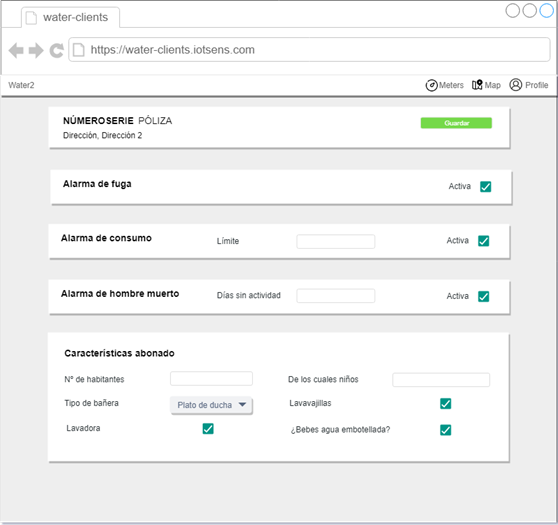
\includegraphics [scale=1] {images/prototipo/imagen5.png}
 \caption{Prototipo del formulario de datos adicionales del contador} \label{fig:prototipo5}
 \end{figure}
 
 \begin{figure}[h]
 \centering
 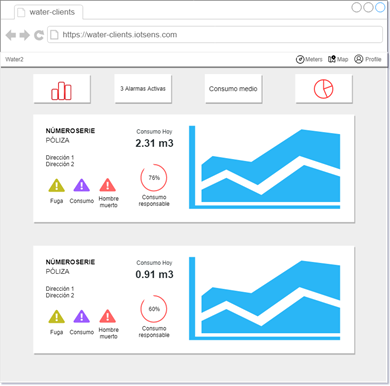
\includegraphics [scale=1] {images/prototipo/imagen6.png}
 \caption{Prototipo del listado de contadores} \label{fig:prototipo6}
 \end{figure}


\end{document}
